\documentclass[superscriptaddress, twocolumn, prx, longbibliography, nofootinbib]{revtex4-1}
\usepackage{amsmath, amssymb, color, graphicx, stmaryrd, wasysym, esint}
\definecolor{linkcolor}{rgb}{0,0,0.6} 
\usepackage[pdftex,colorlinks=true,
	pdfstartview = FitV,
	linkcolor    = linkcolor,
	citecolor    = linkcolor,
	urlcolor     = linkcolor,	
	hyperindex   = true,
	hyperfigures = false]{hyperref}

\newcommand{\dd}{\text{d}}
\newcommand{\ee}{\text{e}}
\newcommand{\ii}{\text{i}}
\newcommand{\tn}[1]{{\color{blue}#1}}


% ===============================================================================


\begin{document}

\title{How dissipation constrains fluctuations in nonequilibrium liquids:\\Diffusion, structure and biased interactions}
\author{Laura Tociu}
\affiliation{James Franck Institute, University of Chicago, Chicago, IL 60637}
\affiliation{Department of Chemistry, University of Chicago, Chicago, IL 60637}

\author{\'Etienne Fodor}
\affiliation{DAMTP, Centre for Mathematical Sciences, University of Cambridge, Wilberforce Road, Cambridge CB3 0WA, UK}

\author{Takahiro Nemoto}
\affiliation{Philippe Meyer Institute for Theoretical Physics, Physics Department, \'Ecole Normale Sup\'erieure \& PSL Research University, 24, rue Lhomond, 75231 Paris Cedex 05, France}

\author{Suriyanarayanan Vaikuntanathan}
\affiliation{James Franck Institute, University of Chicago, Chicago, IL 60637}
\affiliation{Department of Chemistry, University of Chicago, Chicago, IL 60637}

\begin{abstract}

The dynamics and structure of nonequilibrium liquids, driven by non-conservative forces which can be either external or internal, generically hold the signature of the net dissipation of energy in the thermostat. Yet, disentangling precisely how dissipation changes collective effects remains challenging in many-body systems due to the complex interplay between driving and interparticle interactions. First, we combine explicit coarse-graining and stochastic calculus to obtain simple relations between diffusion, density correlations and dissipation in nonequilibrium liquids. Based on these results, we consider large-deviation biased ensembles where trajectories mimic the effect of an external drive. The choice of the biasing function is informed by the connection between dissipation and structure derived in the first part. Using analytical and computational techniques, we show that biased trajectories effectively renormalizes interactions in a controlled manner, thus providing intuition on how driving forces can lead to spatial organization, with potential relevance for complex self-assembly. Altogether, our results show how tuning dissipation provides a route to alter the structure and dynamics of liquids and soft materials.

\end{abstract}

\maketitle

% ===============================================================================


\section{Introduction}

Nonequilibrium forces can drive novel and specific pathways to modulate phase transitions and self-assembly in materials. The close connection between the net dissipation of energy, powered by these forces, internal transport and spatial organization is especially apparent in living systems~\cite{Toyabe2010, Ahmed2016, Battle604, Mura2018}. As an example, the flagella motors of {\it E. Coli} exhibit a unique phenomenology combining ultra-sensitive response, adaptation, and motor restructuring as a function of the applied load~\cite{Lele2013, Lan2012, Wang2017}. Moreover, {\it in vivo} studies of the cellular cytoskeleton, as well as {\it in vitro} experiments on reconstituted systems, have also shown that motor-induced forces control a large variety of functionality in the cell~\cite{Silva2011, Sanchez2012, Blanchoin2014, Murrell2015, Decamp2015}.


To elucidate the role of nonequilibrium forces in materials, it is crucial to examine how dissipation affects the emerging dynamics and structure. 
While equilibrium features are well established, progress in controlling systems with sustained dissipation has been hampered by a lack of general principles~\cite{Cates2015, Solon2015a, Nguyen2016, Fodor2016, Murugan2017, Nardini2017, Nguyen2018}. {In this context}, minimal models of active and driven systems provide analytically and numerically tractable test beds to investigate the interplay between dissipation and material properties far from equilibrium~\cite{Marchetti2013, Han2016, Bechinger2016, delJunco2018, Marchetti2018}. They have illustrated, for instance, how nonequilibrium driving can induce phase transitions and excite novel collective responses in soft media~\cite{Vicsek1995, Tailleur2008, Han2016, Nguyen2016, VanZuiden2016}. Recent theoretical work has proposed extending equilibrium concepts to active media, such as the definition of pressure~\cite{Takatori2015, Solon2015a}, to rationalize their phenomenology~\cite{Solon2018, Solon2018b}. Others have striven to obtain stationary properties of active matter through perturbation close to equilibrium~\cite{Farage2015, Nardini2017, Brader2017}, inspired by other approaches on driven systems~\cite{McLennan1959, Komatsu2008, Maes2009, Maes2010}.


To investigate how dissipation controls emerging behavior, yet another approach {has focused on} introducing a bias in dynamical ensembles. Using large deviation techniques, trajectories are conditioned to promote atypical realizations of the dynamics~\cite{Touchette2009, Jack2010}. {Such techniques have been used}, for instance, to investigate the role of dynamical heterogeneities in glassy systems~\cite{garrahan2007, Hedges2009, Pitard2011, Speck2012, Bodineau2012a, Limmer2014, Nemoto2017} and soliton solutions in high-dimensional chaotic chains~\cite{tailleur2007probing, laffargue2013}. More recently, it has been shown that changing dissipation, through a dynamical bias, strongly affects the internal transport and the density fluctuations of nonequilibrium liquids~\cite{Cagnetta2017, Nemoto2019}, thus confirming that controlling dissipation is indeed a fruitful route to tailoring material properties. {In spite of these advances}, anticipating the emergent dynamics and structure of biased nonequilibrium systems is still challenging in the presence of many-body interactions~\cite{Chetrite2013, Jack2010}, so that precise control has remained elusive so far in this context. {Consequently}, any generic principle rationalizing spatial organization in terms of dissipation is still lacking.


In this paper, we explore how dissipation affects the dynamics and structure of many-body diffusive systems. First, we consider in Sec.~\ref{sec:method} an assembly of Brownian particles where only a subset is driven by an external force. We mainly focus on instances where the fraction of driven particles is less than the fraction of undriven particles, so that driven and undriven particles are respectively referred to as {\it tracer} and {\it bath} particles. Using the diffusion coefficient of a tagged tracer particle and the density correlations between tracer and bath particles, we connect dissipation to liquid properties. At variance with~\cite{delJunco2018}, our prediction for diffusion follows from a systematic coarse-graining with explicit dependence in terms of microscopic details~\cite{Dean1996, Demery2011, Demery2014}. Importantly, we put forward a generic relation between density correlations and dissipation valid for an arbitrary driving force: this is our first main result. It opens the door to estimating dissipation directly from the liquid structure, at variance with previous approaches based either on perturbing the system~\cite{Harada2005, Mizuno2007, Visco2015, Turlier2016, Ahmed2018} or on analyzing trajectories and currents in phase space~\cite{Battle604, Gingrich2017, Roldan2018, Parrondo2018, Li2018}. We illustrate this with numerical simulations for which dissipation is quantified by the deviation from equilibrium tracer-bath correlations. Altogether, these results clarify how nonequilibrium forces affect the transport and structure of the liquid, thus showing how liquid properties can be modified at the cost of energy dissipation.


Motivated by these results, and to provide concrete intuition for how particular configurations can be stabilized by nonequilibrium forces, we investigate in Sec.~\ref{sec:bias} the emerging structure of Brownian particles subject to a dynamical bias. The explicit form of the bias is inspired by the results of Sec.~\ref{sec:method} connecting dissipation to many-body interactions. Using analytical calculations and numerical simulations based on the cloning algorithmm~\cite{Giadina2006, tailleur2007probing, Hurtado2009, Nemoto2016, Ray2018, Klymko2018, Brewer2018}, we show that biased sampling trajectories can be used to renormalize any specific interparticle interaction in a multi-component liquid. The rare noise fluctuations sampled with dynamical bias effectively drive the system away from typical behavior~\cite{garrahan2007, Hedges2009, Jack2010, Pitard2011, Speck2012, Bodineau2012a, Chetrite2013, Limmer2014, Nemoto2017}. Such noise realizations can then serve as proxies of how to control the dynamics by applying an external force with complex protocols. Overall, our results lay the groundwork for precise control of the emerging structure in many-body diffusive nonequilibrium systems. Indeed, {given the ability to control and modify any desired interparticle interaction in a multi-component system}, our results could potentially lead to design principles for addressable self-assembly in
nonequilibrium conditions.


% ===============================================================================


\section{Dissipation and liquid properties}\label{sec:method}

In this Section, we provide a series of relations between energy dissipation and liquid properties in nonequilibrium liquids. Specifically, we consider interacting Brownian particles where a specific set of particles $\Omega$ is driven by a non-conservative forces ${\bf F}_{{\rm d},i}$:
\begin{equation}\label{eq:dyn}
	\gamma\dot{\bf r}_i = \delta_{i\in\Omega}{\bf F}_{{\rm d},i} - \nabla_i \sum_j v({\bf r}_i-{\bf r}_j) + {\boldsymbol\xi}_i ,
\end{equation}
where $\delta_{i\in\Omega}=1$ if $i\in\Omega$ and $\delta_{i\in\Omega}=0$ otherwise. The driven particles belonging to the set $\Omega$ are referred to as {\it tracers}, and others as {\it bath} particles. The fluctuating term ${\boldsymbol\xi}_i$ is a zero-mean Gaussian white noise with correlations $\langle\xi_{i\alpha}(t)\xi_{j\beta}(0)\rangle=2\gamma T\delta_{ij}\delta_{\alpha\beta}\delta(t)$, where $\gamma$ and $T$ respectively denote the damping coefficient and the bath temperature, with the Boltzmann constant set to unity ($k_{\rm B}=1$). 

\subsection{Deterministic and active driving forces}
\label{sec:map}
In what follows, we consider two types of driving forces: (i)~where a subset of particles is driven by an external force all following the same deterministic protocol, and (ii)~where each particle in the chosen set $\Omega$ is driven by an independent noise term. Building on recent work~\cite{Han2016, delJunco2018}, the case (i) of external forces is derived from a time-periodic protocol identical for every tracer, given in two dimensions by
\begin{equation}\label{eq:theta}
	{\bf F}_{\rm d}(t) = f \big[\sin(\omega t) \hat{\bf e}_x + \cos(\omega t)\hat{\bf e}_y \big] ,
\end{equation}
where $f$ and $\omega$ are respectively the amplitude and the frequency of the drive, such as the drive persistence reads $\tau=2\pi/\omega$. The relative strength of the drive is given by the P\'eclet number $\text{Pe} = \sigma f/T$, where $\sigma$ is the typical particle size~\cite{Han2016, delJunco2018}. In the absence of interactions ($v=0$), the average position of driven tracers follows a periodic orbit, describing a circle in two dimensions. In contrast, the case (ii) of internal forces corresponds to random forces akin to the ones modelling self-propulsion in active liquids~\cite{Fily2012, Redner2013, Maggi2015}. Specifically, we use a set of zero-mean Gaussian noises uncorrelated with ${\boldsymbol\xi}_i$ with correlations 
\begin{equation}\label{eq:theta_ac}
	\langle F_{{\rm d},i\alpha}(t) F_{{\rm d},j\beta}(0) \rangle = \delta_{ij}\delta_{\alpha\beta} f^2 {\rm e}^{-|t|/\tau} .
\end{equation}
The parameters $f$ and $\tau$ respectively control the amplitude and the persistence of fluctuations. As detailed below, ~\eqref{eq:theta_ac} can be obtained by combining various deterministic driving protocols in~\eqref{eq:theta} with amplitudes and frequencies chosen from a specific distribution. 

%the relations between dissipation and liquid properties bare some analogies when considering either~\eqref{eq:theta} or~\eqref{eq:theta_ac}, thus allowing for a consistent treatment for a large class of nonequilibrium liquids.

%\subsection{Activity as a disordered drive}\label{sec:map}

%As a first step, we put forward an explicit mapping of a specific deterministic disordered drive into a corresponding noise term. To this end, we consider

% -------------------------------------------------------------------------------

In particular, consider a generalized version of the deterministic force~\eqref{eq:theta} where now each particle $i$ is subjected to an independent drive. The period of the orbit is determined by a series of $n$ oscillators with identical frequencies for all particles, yet independent amplitudes:
\begin{equation}\label{eq:theta_dis}
	{\bf F}_{{\rm d}, i}(t) = \frac{f}{\sqrt{n}} \sum_{a=1}^n \big[ {\bf A}_{ai} \cos(\omega_a t) + {\bf B}_{ai} \sin(\omega_a t) \big] .
\end{equation}
The drive disorder is implemented by taking the oscillator amplitudes as uncorrelated zero-mean Gaussian variables with unit variance:
\begin{equation}
	\langle A_{ai\alpha}A_{bj\beta}\rangle_{\rm d} = \delta_{ab}\delta_{ij}\delta_{\alpha\beta} = \langle B_{ai\alpha}B_{bj\beta}\rangle_{\rm d} ,
\end{equation}
where $\langle\cdot\rangle_{\rm d}$ denotes an average over the disorder. It follows that ${\bf F}_{{\rm d},i}$ is a also Gaussian process with zero mean and correlations given by
\begin{equation}
	\langle F_{{\rm d},i\alpha} (t) F_{{\rm d},j\beta}(0) \rangle_{\rm d} = \delta_{ij} \delta_{\alpha\beta} \frac{f^2}{n} \sum_{a=1}^n \cos (\omega_a t) .
\end{equation}
In the limit of a large number of oscillators ($n\gg1$), we express these correlations in terms of the density of driving frequencies $\phi$ as
\begin{equation}\label{eq:drive_corr}
	\langle F_{{\rm d},i\alpha} (t) F_{{\rm d},j\beta}(0) \rangle_\text{d} \underset{n\gg1}{=} \delta_{ij} \delta_{\alpha\beta} f^2 \int \phi(\omega') \ee^{\ii\omega'|t|} \frac{\dd\omega'}{2\pi} .
\end{equation}
This establishes that, in the limit of many oscillators, the deterministic drive~\eqref{eq:theta_dis} with disordered amplitude is equivalent into a noise term with spectrum $\phi$. In particular, by choosing $\phi(\omega') = 2\tau/ \big[1+(\omega'\tau)^2\big]$, the drive correlations~\eqref{eq:drive_corr} reproduce exactly the ones of the random force in~\eqref{eq:theta_ac}.


To illustrate the relevance of this mapping, we simulate numerically the many-body dynamics~\eqref{eq:dyn} where every particle is subject a disordered drive of the form~\eqref{eq:theta_dis}. We use the potential $v({\bf r})=v_0(1-|{\bf r}|/\sigma)^2\Theta(\sigma-|{\bf r}|)$, where $\Theta$ denotes the Heaviside step function, which sets purely repulsive interactions. To implement numerically the disorder in driving, it is sufficient to sample the amplitudes $\{{\bf A}_{ai}, {\bf B}_{ai}\}$ and frequencies $\{\omega_i\}$ at initial time. In the regime of high persistence $\tau$ and large average density $\rho_0$, we observe the spontaneous formation of clusters up to a complete phase separation at large time, see Fig.~\ref{fig0}. This is analogue to the motility-induced phase separation commonly reported in standard models of active particles~\cite{Tailleur2008, Cates2015}. Interestingly, it appears in our case even in the absence of fluctuations ($T=0$), namely for a purely deterministic set of equations. In short, we thus demonstrate that the disordered drive alone reproduces the emerging physics of active systems. 

By deriving our results for both ~\eqref{eq:theta} and ~\eqref{eq:theta_ac}, we can hence demonstrate that our work has broad applicability \textendash from systems being driven by deterministic time dependent fields to active matter like systems. 

\begin{figure}
	\centering
	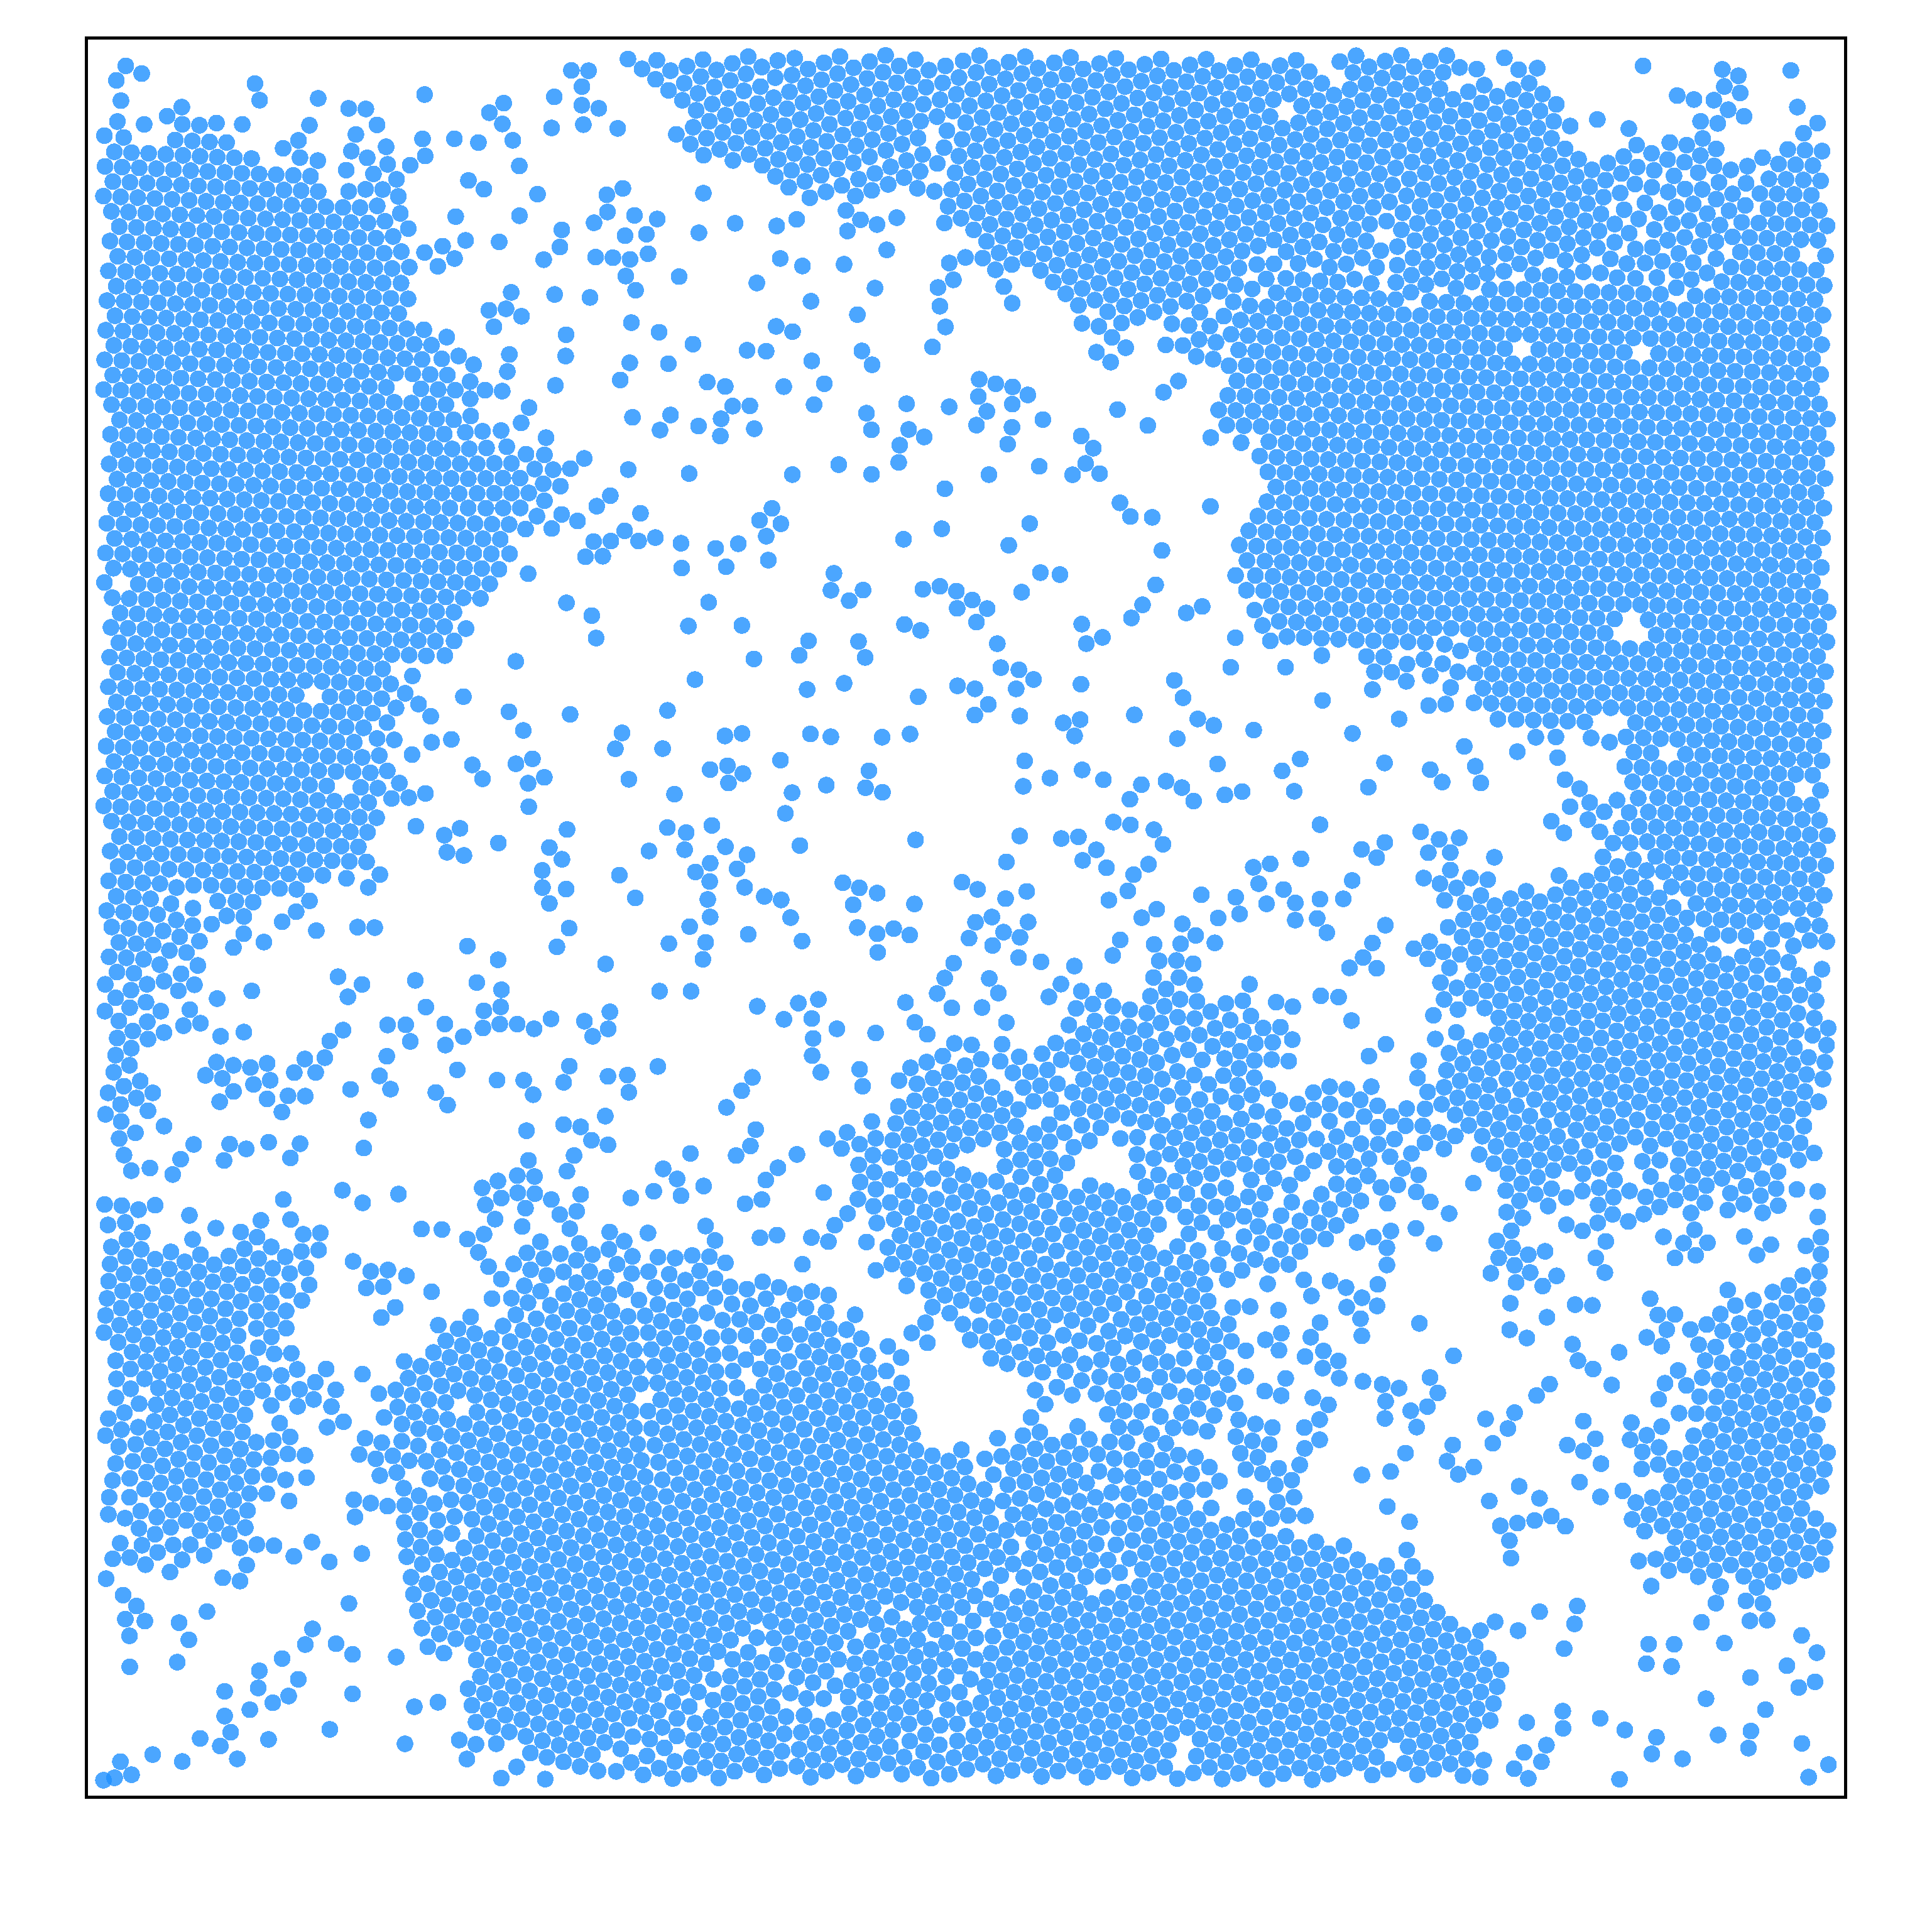
\includegraphics[width=.8\columnwidth]{fig0.pdf}
	\caption{\label{fig0}
		Snapshot of particles subjected to a disordered drive. A phase separation emerges which is analogue to the motility-induced phase separation of active particles~\cite{Tailleur2008, Cates2015}. Simulation details in Appendix~\ref{app:simu} and movie in~\cite{movie}.
	}
\end{figure}


% -------------------------------------------------------------------------------


\subsection{Dissipation controls tracer diffusion}\label{sec:diff}

To connect tracer diffusion with dissipation, we first describe the dynamics of undriven particles in terms of a coarse-grained variable. Using standard techniques, the dynamics of the density field $\rho({\bf r},t) = \sum_{i\not\in\Omega}\delta[{\bf r}-{\bf r}_i(t)]$ can be written as a non-linear Langevin equation~\cite{Dean1996}. In the regime of weak interactions, the density fluctuations $\delta \rho({\bf r},t ) = \rho({\bf r}, t) - \rho_0$ around the average density $\rho_0$ are Gaussian and captured by the following Hamiltonian~\cite{Chandler1993, Demery2014, Kruger2017}:
\begin{equation}
	\begin{aligned}
		{\cal H} &= \frac{T}{2} \int \delta \rho ({\bf r}) K({\bf r} - {\bf r}') \delta \rho ({\bf r}') \dd{\bf r}\dd{\bf r}'
		\\
		&\quad + \int \sum_{i\in\Omega} v({\bf r}-{\bf r}_i) \rho({\bf r}) \dd{\bf r} ,
	\end{aligned}
\end{equation}
where $K({\bf r})= \delta({\bf r})/\rho_0 + v({\bf r})/T$. The conserved density dynamics reads
\begin{equation}\label{eq:EvolutionField}
	\begin{aligned}
		\frac{\partial \delta \rho({\bf r}, t)}{\partial t} &= D_{\rm G} \nabla^2 \int K({\bf r}-{\bf r}') \delta \rho({\bf r}', t) \dd{\bf r}'
		\\
		&\quad + \frac{1}{\gamma_{\rm G}} \nabla^2 \sum_{i\in\Omega}v({\bf r}-{\bf r}_i(t)) + \nabla \cdot {\boldsymbol\Lambda}({\bf r},t) ,
	\end{aligned}
\end{equation}
where $D_{\rm G} = \rho_0 T/\gamma$ and $\gamma_{\rm G}=\gamma/\rho_0$ are respectively the field diffusion coefficient and the field damping coefficient. The term $\boldsymbol\Lambda$ is a zero-mean Gaussian white noise with correlations $\langle \Lambda_\alpha({\bf r}, t) \Lambda_\beta({\bf r}', t') \rangle = 2 D_{\rm G} \delta_{\alpha\beta}\delta({\bf r} - {\bf r}')\delta(t-t')$.


Owing to the linearity of the density dynamics~\eqref{eq:EvolutionField}, it can be readily written in Fourier space $\delta\rho({\bf q},t)=\int\rho({\bf r},t){\rm e}^{-{\rm i}{\bf q}\cdot{\bf r}} {\rm d}{\bf r}$ as
\begin{equation}\label{eq:FourierEvolutionField}
	\begin{aligned}
		\frac{\partial \delta \rho({\bf q},t)}{\partial t} &= - |{\bf q}|^2 D_{\rm G} K({\bf q}) \delta \rho({\bf q},t)
		\\
		&\quad - |{\bf q}|^2 \frac{v({\bf q})}{\gamma_{\rm G}} \sum_{j\in\Omega}\ee^{-\ii {\bf q} \cdot {\bf r}_j(t)} + \ii{\bf q}\cdot{\boldsymbol\Lambda} ({\bf q},t) ,
	\end{aligned}
\end{equation}
so that the field dynamics can be directly solved as
\begin{equation}\label{eq:rho}
	\begin{aligned}
		\delta\rho({\bf q},t) &= \int_{-\infty}^t \dd s \ee^{-D_{\rm G} |{\bf q}|^2 K({\bf q})(t-s)}
		\\
		&\quad\times \bigg[ \ii{\bf q} \cdot {\boldsymbol\Lambda}({\bf q},s) - |{\bf q}|^2 \frac{v({\bf q})}{\gamma_{\rm G}} \sum_{j\in\Omega}\ee^{-\ii {\bf q}\cdot {\bf r}_j(s)}\bigg] .
	\end{aligned}
\end{equation}
Considering the limit of dilute driven tracers, where interactions among them are negligible, their dynamics reads
\begin{equation}\label{eq:EvolutionTracer}
	\gamma\dot{\bf r}_j = {\bf F}_\text{d} + {\boldsymbol\xi_j} - \int_{\bf q} \ii{\bf q} v(-{\bf q})\ee^{\ii{\bf q} \cdot {\bf r}_j(t)} \delta \rho({\bf q}, t) ,
\end{equation}
with $\int_{\bf q}=\int\dd{\bf q}/(2\pi)^d$ and $d$ referring to spatial dimension. As a result,~\eqref{eq:rho} and~\eqref{eq:EvolutionTracer} provide closed time-evolution equations for tracers only. It should only be valid for weak interactions {\it a priori}, yet previous works have shown that it remains qualitatively relevant even beyond this regime in practice~\cite{Demery2015, Martin2018, Demery2019}. Indeed, Gaussian field theories for density fluctuations provide a very good description of simple liquids~\cite{Chandler1993}.


To characterize the transport properties of the liquid in the presence of driving forces, our first goal is to obtain an explicit expression, in terms of microscopic details, for the tracer diffusion coefficient:
\begin{equation}
	D = \underset{t\to\infty}{\lim} \frac{1}{2dt} \big\langle \big[\langle{\bf r}_i(t)\rangle-{\bf r}_i(t)\big]^2 \big\rangle .
\end{equation}
We aim to explore connections between $D$ and dissipation, which is defined from stochastic thermodynamics as the power of the forces exerted by all tracers on solvent: ${\cal J} = \sum_i\langle\dot{\bf r}_i\cdot(\gamma\dot{\bf r}_i-{\boldsymbol\xi}_i)\rangle$, where $\cdot$ denotes a Stratonovich product~\cite{Sekimoto1998, Seifert2012}. Substituting the dynamics~\eqref{eq:dyn}, the dissipation coincides with the power of driving forces: ${\cal J} = \sum_{i\in\Omega}\langle\dot{\bf r}_i\cdot{\bf F}_{{\rm d},i}\rangle$, and it can be further separated into free-motion and interaction contributions as ${\cal J} = f^2/\gamma - \dot w$, where the {\it rate of work} reads
\begin{equation}\label{eq:work}
	\dot w = \frac{1}{\gamma} \sum_{i\in\Omega,j}\big\langle {\bf F}_{{\rm d},i}\cdot\nabla_iv({\bf r}_i-{\bf r}_j)\big\rangle.
\end{equation}
Given that $\dot w$ is the only non-trivial contribution to dissipation, connecting diffusion and dissipation simply amounts to expressing $D$ in terms of $\dot w$.


Deriving transport coefficients in nonequilibrium many-body systems, whose collective effects result from the complex interplay between interaction and driving forces, is a notoriously difficult task~\cite{Voituriez2016, Brady2017, Stenhammar2017, Tailleur2017, Illien2018}. We set up a proper perturbation scheme by scaling the pair potential $v$ with a small dimensionless parameter $h\ll1$ which controls the coupling between tracer and bath. In Appendix~\ref{app:diff}, we obtain some explicit expressions for $D$ and $\dot w$ to quadratic order in $h$ and in the scaled driving amplitude $\rm Pe$.


First, we discuss the case of the external driving~\eqref{eq:theta}, and we focus on the limits of small and large driving frequency, respectively $\omega\tau_{\rm r}\ll 1$ and $\omega\tau_{\rm r}\gg 1$, where the relaxation time scale $\tau_{\rm r}=(D_{\rm G}/\sigma^2)K(|{\bf q}|=1/\sigma)$ is set by density diffusion over the tracer size $\sigma$. First, at high frequencies $\omega\tau_{\rm r}\gg 1$, the rate of work $\dot w$ and the deviation from equilibrium diffusion $D-D_{\rm eq}$, where $D_{\rm eq}$ is the diffusion coefficient for ${\rm Pe}=0$, are given by
\begin{equation}\label{eq:large}
	\begin{aligned}
		\dot w &= \Big(\frac{h{\rm Pe}}{\omega}\Big)^2 \cdot \frac{(T/\sigma)^2}{d\gamma^3} \int_{\bf q} |{\bf q}|^4 |v({\bf q})|^2 \frac{1 + \rho_0K({\bf q})}{K({\bf q})} ,
		\\
		D-D_{\rm eq} &= \Big(\frac{h{\rm Pe}}{\omega}\Big)^2 \cdot \frac{T /\sigma^2}{d\gamma^3} \int_{\bf q}\frac{|{\bf q}|^2 |v({\bf q})|^2 } {K({\bf q})\big[1 + \rho_0 K({\bf q})\big]} .
	\end{aligned}
\end{equation}
In the opposite limit of low frequencies $\omega\tau_{\rm r}\ll 1$, we get
\begin{equation}\label{eq:small}
	\begin{aligned}
		\dot w &= \frac{(h{\rm Pe})^2}{d\gamma\sigma^2} \int_{\bf q} \frac{|v({\bf q})|^2}{K({\bf q})\big[1 + \rho_0K({\bf q})\big]} ,
		\\
		D - D_{\rm eq} &= \frac{5(h{\rm Pe})^2}{d\gamma T\sigma^2} \int_{\bf q} \frac{|v({\bf q})|^2}{|{\bf q}|^2K({\bf q})\big[1 + \rho_0K({\bf q})\big]^3} .
	\end{aligned}
\end{equation}
Both $\dot w$ and $D-D_{\rm eq}$ are now independent of the driving frequency $\omega$. As a result, our perturbation theory hence shows that scalings of $\dot w$ and $D-D_{\rm eq}$ are identical, both in terms of the drive amplitude $\rm Pe$ and of its frequency $\omega$, in asymptotic frequency regimes. Note that the scaled rate of work $\gamma\dot w/f^2$ coincides with the reduced equilibrium diffusion $\gamma D_{\rm eq}/T-1$ to this order~\cite{Demery2011, Demery2014}, as expected from linear response.


The case of the internal driving with correlations~\eqref{eq:theta_ac} follows by using the mapping between disordered drive and active forcing in Sec.~\ref{sec:map}. In practice, we first derive the diffusion coefficient $D$ and the rate of work $\dot w$ for the driving force~\eqref{eq:theta_dis} at fixed disorder, as a straightforward generalization of the external driving case, and we then average over the disorder. At small persistence $\tau\ll\tau_{\rm r}$, we get
\begin{equation}\label{eq:small_tau}
	\begin{aligned}
		\dot w &=  \frac{\tau T(h{\rm Pe})^2}{d(\sigma\gamma)^2} \int_{\bf q} \frac{|{\bf q}|^2 |v({\bf q})|^2}{K({\bf q})} ,
		\\
		D-D_{\rm eq} &= \frac{3\tau(h{\rm Pe})^2}{d(\sigma\gamma)^2} \int_{\bf q}\frac{|v({\bf q})|^2 } {K({\bf q})\big[1 + \rho_0 K({\bf q})\big]^2} .
	\end{aligned}
\end{equation}
In contrast, the large persistence limit $\tau\gg\tau_{\rm r}$ yields the same results as for the low frequencies regime of external driving, namely the expressions~\eqref{eq:small}. Indeed, the force ${\bf F}_{{\rm d},i}$ has a constant direction in such a limit, and the difference between internal and external drivings, which respectively correspond to independent or similar directions for each tracer, is irrelevant in the dilute limit.


When the size $a$ of the bath particles is significantly smaller than the tracer size $\sigma\gg a$, which amounts to setting different pair potential $v$ for bath-bath and for bath-tracer interactions, one can safely neglect the variation of $K({\bf q})$ in~(\ref{eq:large}-\ref{eq:small_tau}), so that $K({\bf q}) \simeq K(|{\bf q}|=1/a)$. Then, in both regimes $\omega\tau_{\rm r}\gg 1$ ($\tau\ll\tau_{\rm r}$) and $\omega\tau_{\rm r}\ll 1$ ($\tau\gg\tau_{\rm r}$), the renormalization of the diffusion coefficient $D-D_{\rm eq}$ can be simply written in terms of the rate of work $\dot w$ for ${\rm Pe}\ll1$ as
\begin{equation}\label{eq:work_D}
	\frac{D-D_{\rm eq}}{\sigma^2} \sim \frac{\dot w}{T} .
\end{equation}
Thus, the excess rate at which tracers move over their own size compared to equilibrium, set by the lhs of~\eqref{eq:work_D}, is controlled by the rate at which work is applied on tracers by nonequilibrium forces, set by the rhs of~\eqref{eq:work_D}. The proportionality factor depends on the details of interactions and of density fluctuations. Interestingly, this result is valid both for internal and external drivings. It corroborates numerical observations obtained previously in a system where composition-dependent diffusion constants can lead to phase transitions~\cite{delJunco2018}.


% -------------------------------------------------------------------------------


\subsection{Dissipation sets density correlations}\label{sec:struc}

We now explore how dissipation relates with static density correlations of the liquid. To this end, we treat undriven bath particles without any approximation in what follows, instead of relying on the Gaussian density field theory for $\delta\rho$ as we did above, and we consider an arbitrary set of driving forces ${\bf F}_{{\rm d},i}$. In equilibrium, the liquid structure can be derived from a hierarchy of equations for density correlations, whose explicit form reflects the steady-state condition on the many-body distribution function~\cite{Hansen2013}. In our settings, steady-state conditions should now provide modified equations for density correlations, which can potentially make apparent the connection with dissipation.


This motivates us to consider the average rate at which the potential $U = \sum_{i\in\Omega,j} v({\bf r}_i-{\bf r}_j)$ changes, which can be written using It\^o calculus as
\begin{equation}
	\gamma\langle\dot U \rangle = \sum_{i\in\Omega,j} \big\langle\big[\gamma(\dot{\bf r}_i - \dot{\bf r}_j) + 2 T \nabla_i\big] \circ \nabla_i v({\bf r}_i-{\bf r}_j)\big\rangle ,
\end{equation}
where $\circ$ denotes an It\^o product. Substituting the dynamics~\eqref{eq:dyn} and using $\langle{\boldsymbol\xi}_i\circ\nabla_i v\rangle=0$, we get
\begin{equation}\label{eq:dotU}
	\begin{aligned}
		&\gamma\langle\dot U \rangle = \sum_{i\in\Omega,j} \big\langle({\bf F}_{{\rm d},i} + 2 T \nabla_i) \cdot \nabla_i v({\bf r}_i-{\bf r}_j)\big\rangle
		\\
		&\,+ \sum_{i\in\Omega,j,k} \big\langle \big[\nabla_i v({\bf r}_i-{\bf r}_j)\big]\cdot \nabla_k \big[ v({\bf r}_i-{\bf r}_k) - v({\bf r}_j-{\bf r}_k) \big] \big\rangle ,
    \end{aligned}
\end{equation}
where the $k$-sum runs over all particles. Then, using the steady-state condition $\langle\dot U \rangle=0$ and identifying the rate of work from its definition~\eqref{eq:work}, we deduce that $\dot w$ can be written in terms of density correlations as
\begin{equation}\label{eq:balance}
	\begin{aligned}
		&\gamma\dot w = 2\rho_0 \int g({\bf r}) \big[(\nabla v({\bf r}))^2 - T \nabla^2 v({\bf r})\big] \dd{\bf r} ,
		\\
		&\, + \rho_0^2 \iint\big[ g_{3a}({\bf r}, {\bf r}') + g_{3b}({\bf r}, {\bf r}')\big]  \big[\nabla v({\bf r})\big] \cdot \big[\nabla v({\bf r}')\big] \dd{\bf r} \dd{\bf r}' ,
	\end{aligned}
\end{equation}
where
\begin{equation}
	\begin{aligned}
 		g({\bf r}) &= \frac{1}{N} \underset{i\in\Omega,j}{{\sum}'} \big\langle \delta({\bf r}-{\bf r}_i+{\bf r}_j)\big\rangle ,
		\\
 		g_{3a}({\bf r},{\bf r}') &= \frac{1}{N^2} \underset{i\in\Omega,j,k}{{\sum}'} \big\langle \delta({\bf r}-{\bf r}_i+{\bf r}_j) \delta({\bf r}'-{\bf r}_i+{\bf r}_k)\big\rangle ,
		\\
 		g_{3b}({\bf r},{\bf r}') &= \frac{1}{N^2} \underset{i\in\Omega,j,k}{{\sum}'} \big\langle \delta({\bf r}-{\bf r}_i+{\bf r}_j) \delta({\bf r}'-{\bf r}_j+{\bf r}_k)\big\rangle ,
	\end{aligned}
\end{equation}
and $\sum'$ denotes a sum without the overlap of indices: $i\neq j$, $k\neq i$ and $k\neq j$. The power balance~\eqref{eq:balance}, valid for an arbitrary driving, either internal or external, is our first main result.


In practice, it reflects how density correlations adapt to the presence of nonequilibrium forces. For a vanishing rate of work ($\dot w = 0$), one recovers the first order of the equilibrium Yvon-Born-Green hierarchy, in its integral form, for two-component fluids~\cite{Hansen2013}. At finite rate of work ($\dot w\neq0$), the relation between the two-body correlation $g$ and the three-body terms $\{g_{3a},g_{3b}\}$ is now implicitly constrained by dissipation. A direct implication is that the rate of work can now be inferred simply by measuring static density correlations, provided that the pair-wise interaction potential is known, for a given driven liquid. Importantly, such an approach does not require any invasive methods based on comparing fluctuations and response~\cite{Harada2005, Mizuno2007, Visco2015, Turlier2016, Ahmed2018}, and it does not rely on a detailed analysis of particle trajectories~\cite{Roldan2018, Parrondo2018} or currents in phase space~\cite{Gingrich2017, Li2018}, whose experimental implementation can require elaborate techniques~\cite{Battle604, Mura2018}.


\begin{figure}
	\centering
	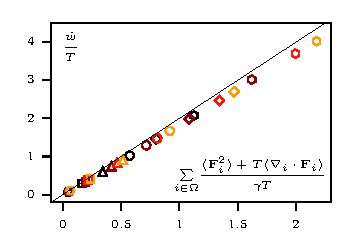
\includegraphics[width=\linewidth]{fig1.pdf}
	\caption{\label{fig:fig1}
		Parametric plot of the rate of work $\dot w/T$ and of the statistics of bath-tracer forces $\sum_{i\in\Omega}\big[\langle{\bf F}_i^2\rangle + T\langle\nabla_i\cdot{\bf F}_i\rangle\big]/\gamma T$ for a dilute fraction of driven particles ($10\%$). The solid line refers to the approximate relation~\eqref{eq:approx}. The satisfying agreement with numerical data indicates that dissipation can be estimated by only measuring bath-tracer forces.
		Simulation details in Appendix~\ref{app:simu}. Parameters: $\tau/\tau_{\rm r}=20$ (black), $30$ (brown), $40$ (red), $50$ (orange); ${\rm Pe}=6$ ($\hexagon$), $12$ ($\boxempty$), $18$ ({\large$\vartriangle$}), $24$ ({$\Circle$}), $30$ (${\Diamond}$), $36$ ($\varhexagon$).
	}
\end{figure}


However, the power balance~\eqref{eq:balance} is not straightforward to test, either numerically or experimentally, due to the three-body correlations. In equilibrium, where tracer and bath particles are indistinguishable, we get $g_{3a}=g_{3b}$. Assuming that this remains approximately valid in the driven case for a dilute fraction of tracers, the rate of work can simply be written in terms of the force exerted on a tracer ${\bf F}_i =- \sum_j\nabla_iv({\bf r}_i-{\bf r}_j)$ as
\begin{equation}\label{eq:approx}
	\gamma\dot w \simeq 2\sum_{i\in\Omega} \big[ \big\langle{\bf F}_i^2\big\rangle + T \big\langle\nabla_i\cdot{\bf F}_i\big\rangle \big] .
\end{equation}
To probe the validity of this result, we simulate the dynamics~\eqref{eq:dyn} with a fraction $f=0.1$ of particles being subjected to the driving force. We performed simulations with both (a) the deterministic periodic drive~\eqref{eq:theta} and (b) the active noise drive~\eqref{eq:theta_ac}. Interactions are set by the WCA potential $v({\bf r})=4v_0\big[(\sigma/|{\bf r}|)^{12}-(\sigma/|{\bf r}|)^6\big]\Theta(2^{1/6}\sigma-|{\bf r}|)$~\cite{WCA1971}. Our measurements in Fig.~\ref{fig:fig1} show that~\eqref{eq:approx} is indeed a good approximation at small $\rm Pe$ and small $\tau$, namely when the drive only weakly perturbs the liquid. Besides, up to ${\rm Pe}=36$ and $\tau/\tau_{\rm r}=50$, the relative deviation is at most of about $10\%$. At variance with previous approaches~\cite{Harada2005, Lander2012, Battle604}, which rely on prospecting the whole system, our results demonstrate that dissipation can actually be evaluated with only a small error by considering solely forces acting on tracer: the contribution of forces on other particles is negligible for a dilute fraction of driven tracers.


\begin{figure*}
	\centering
	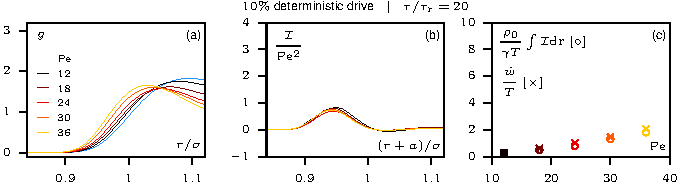
\includegraphics[width=\linewidth]{fig2a.pdf}
	\vskip.5cm
	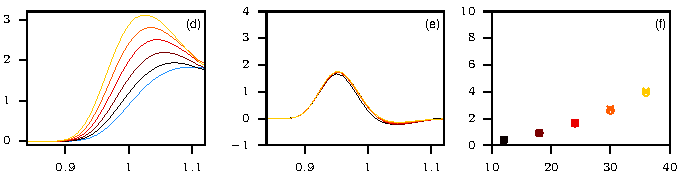
\includegraphics[width=\linewidth]{fig2b.pdf}
	\vskip.5cm
	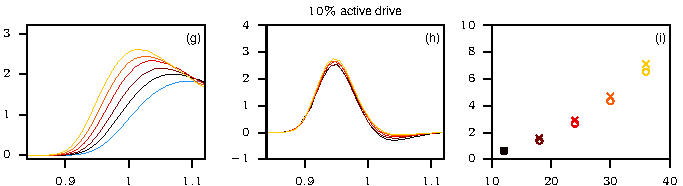
\includegraphics[width=\linewidth]{fig2c.pdf}
	\vskip.5cm
	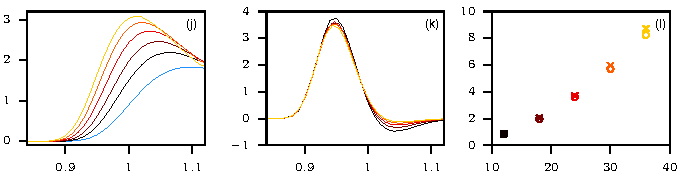
\includegraphics[width=\linewidth]{fig2d.pdf}
	\caption{\label{fig:fig2}
		(Left) Bath-tracer density correlation $g$ as a function of interparticle distance $r/\sigma$. The blue solid line corresponds to the equilibrium correlation function $g_{\rm eq}$ for ${\rm Pe}=0$.
		(Middle) Deviation from equilibrium correlations ${\cal I} = \big[(\nabla v)^2-T\nabla^2v\big](g - g_{\rm eq})$ scaled by ${\rm Pe}^2$ as a function of $r/\sigma$. The data almost collapse into a master curve for a given $\tau/\tau_{\rm r}$.
		(Right) Integrated deviation from equilibrium correlations $(\rho_0/\gamma T)\int{\cal I}({\bf r}){\rm d}{\bf r}$ and rate of work $\dot w/T$ as functions of $\rm Pe$. The former under-estimates $\dot w$ by at most approximately $10\%$, showing that the deviation from equilibrium correlations provides a direct access to dissipation with only a small error.
		Simulation details in Appendix~\ref{app:simu}.
	}
\end{figure*}


To evaluate further the change in liquid structure induced by dissipation, we measure the deviation from equilibrium pair correlations $g-g_{\rm eq}$ due to the driving forces (left column in Fig.~\ref{fig:fig2}). In particular, inspired by the two-body contribution in the power balance~\eqref{eq:balance}, we focus on the observable ${\cal I} = \big[(\nabla v)^2-T\nabla^2v\big](g - g_{\rm eq})$.  At a given $\tau/\tau_{\rm r}$, scaling ${\cal I}$ by ${\rm Pe}^2$ reveals that all curves almost collapse into a master curve for our numerical range ${\rm Pe}\in[12,36]$, as reported in the middle column of Fig.~\ref{fig:fig2}. Given that the rate of work also exhibits such a scaling, this suggests the existence of an underlying relation between $\int{\cal I}({\bf r}){\rm d}{\bf r}$ and $\dot w$. In practice, introducing a factor $\rho_0/\gamma$ provides a satisfactory agreement between them, as shown in the right column of Fig.~\ref{fig:fig2}. In the appendix, we provide some heuristic arguments that explain the connection between ${\cal I}$ and $\dot{w}$. As a result, this empirical relation demonstrates that, for both the periodic drive~\eqref{eq:theta} and the active drive~\eqref{eq:theta_ac} in the dilute limit, the dissipation can actually be directly estimated by comparing driven and equilibrium pair correlations. To probe the effectiveness of our approach in the opposite limit where the entire system is subjected to a drivign force, we performed simulations in which all the particles were driven by the active noise drive~\eqref{eq:theta_ac}. In Fig XXX, we find that the pair correlation functions and dissipation even in a prototypical active matter system can be anticipated or constrained by keeping track of energy flows. 


Overall, the results of this Section illustrate how dissipation affects the transport and structural properties of driven liquids, measured in terms of diffusion coefficient and density fluctuations. These findings motivate the following question: can nonequilibrium forces be tuned to reliably stabilize target configurations? To explore this, we rely in what follows on the framework of large deviation theory. In practice, our strategy amounts to biasing trajectories in terms of dissipation, related to many-body interactions by~\eqref{eq:balance}, to mimic the effect of an external drive. Following this route, our analytical and numerical results provide some concrete intuition for how interactions in a multicomponent system can be controllably renormalized by nonequilibrium forces. Hence, we demonstrate the ability to nucleate structures different from those characteristic of the equilibrium Boltzmann distribution, and thus to help guiding self-assembly even far from equilibrium{~\cite{Bisker2018}}. These results further illustrate the interplay between energy {dissipation} and organization in nonequilibrium many-body settings.



% ===============================================================================


\section{Interactions in biased ensembles}\label{sec:bias}

\tn{We consider a system of interacting Brownian particles without any driving force} 
\begin{equation}\label{eq:dyn_eq}
	\gamma\dot{\bf r}_i = - \nabla_i \sum_j v({\bf r}_i-{\bf r}_j) + {\boldsymbol\xi}_i ,
\end{equation}
where the statistics of the noise term ${\boldsymbol\xi}_i$ is the same as the one in~\eqref{eq:dyn}. 
\tn{The dissipation of this system ${\cal E}$, given as \eqref{eq:balance}, has a zero mean because of the absence of the driving force. 
In order to increase this mean dissipation, we then add a force term 
${\bf F}_i$ to this equation, that includes both inter-particle many-body interactions and a driving force.
As infinitely many ways to define the force exist, increasing the same amount of dissipation does not result in a unique way of forcing. In this section, we select the ``most natural'' forcing among them (more precise meaning is given below) and we study the relation between dissipation and structural properties of driven liquids in this forced system. }


\tn{To introduce the idea of unique forcing, let us consider a set of possible noise realizations in \eqref{eq:dyn_eq}. In each realization, dynamics of the particles are systematically generated according to \eqref{eq:dyn_eq}, whose time-averaged dissipation is deviated from zero in general: some realizations favor to increase the dissipation while some do not, but in average it becomes zero. We then collect the realizations that result in  a specific value of the averaged dissipation bigger than zero. 
In this subset of noise realizations, we look for  ``natural'' ones whose occurrence probabilities are the highest. The dynamics generated by these noise realizations are atypical (largely deviated from the typical dynamics) because of the conditioning on higher dissipation, but ``natural'' in the sense that the probability is the highest in the subset for the same dissipation. In this subset, the noise term in~\eqref{eq:dyn_eq} no longer has zero average, so that we re-define it in terms of a renormalizing force ${\bf F}_i$ as ${\boldsymbol \xi}_i \to {\boldsymbol \xi}_i + {\bf F}_i$. 
This renormalizing force, here we call ``auxiliary force'' according to~\cite{Jack2010,Chetrite2013}, is our target, which has been studied in many theories, e.g., a maximum entropy principle [ ], large deviation principle [ ] or thermodynamic formalism [ ], where applications ranged from glassy systems [ ], non-linear chaotic dynamics [ ], to active matter [ ].


Formally, the auxiliary force and these conditional trajectories are studied by analyzing an exponentially biased ensemble, defined as the dynamical path probability multiplied by an exponential weighting factor $\exp\big[\kappa\int_0^t{\cal E}(s){\rm d}s\big]$, where ${\cal E}(s)$ is a quantity for the conditioning ({\it e.g.}, the dissipation) and $\kappa$ is a conjugate field. Following the thermodynamic formalism~\cite{Touchette2009}, trajectories following this biased path probability are statistically equivalent to those of conditional trajectories, in which the conditional value $\cal E$ and the conjugate field $\kappa$ are related via a Legendre transform. Before analyzing our main problem, relation between dissipation and structural properties of driven liquids, we first introduce how to extract the auxiliary force from the exponentially biased ensemble, by using a simple example in the next subsection.}


% -------------------------------------------------------------------------------


\subsection{{Dynamical bias and external forces}}\label{sec:biasexternal}

To introduce pedagogically our methods, we first show how biasing trajectories can lead to effectively introduce a driving force. Inspired by the role of dissipation in emerging liquid properties, as discussed in Sec.~\ref{sec:method}, we bias the equilibrium dynamics~\eqref{eq:dyn_eq} with the sum of the dissipation and the rate of work, scaled by $T$, that would be produced by applying a constant force ${\bf F}_{\rm d}$ to a subset $\Omega$ of particles:
\begin{equation}\label{eq:eps}
	{\cal E} = \frac{1}{\gamma T}\sum_{i\in\Omega} {\bf F}_{\rm d}\cdot\big[ \gamma\dot{\bf r}_i + \nabla_i V \big] ,
\end{equation}
where $V=(1/2)\sum_{i,j}v({\bf r}_i-{\bf r}_j)$. The path probability ${\cal P}\sim\exp\big[-\sum_i\int_0^t{\mathbb A}_i(s){\rm d}s\big]$ corresponding to this biased ensemble is obtained with standard methods~\cite{Martin1973, Dominicis1975}:
\begin{equation}\label{eq:action_exp}
	{\mathbb A}_i = \frac{1}{4\gamma T} \big[\gamma\dot{\bf r}_i + \nabla_iV\big]^2 - \frac{1}{2\gamma} \nabla^2_iV - \frac{\kappa}{\gamma T} \delta_{i\in\Omega} {\bf F}_{\rm d} \cdot\big[ \gamma\dot{\bf r}_i + \nabla_i V \big] ,
\end{equation}
where the two first terms correspond to the unbiased dynamics~\eqref{eq:dyn_eq}, and the third one to the bias in~\eqref{eq:eps}. It can also be written as
\begin{equation}\label{eq:action}
	{\mathbb A}_i = \frac{1}{4\gamma T} \big[\gamma\dot{\bf r}_i - 2\kappa\delta_{i\in\Omega}{\bf F}_{\rm d} + \nabla_iV\big]^2 - \frac{1}{2\gamma} \nabla^2_iV - \frac{\kappa^2}{\gamma T}\delta_{i\in\Omega}{\bf F}_{\rm d}^2 .
\end{equation}
As a result, given that the last term in~\eqref{eq:action} can be absorbed in a normalization factor, we deduce that the trajectories biased by~\eqref{eq:eps} can be generated, at leading order, in a physical dynamics where the external force $2\kappa{\bf F}_{\rm d}$ is applied to every particle in $\Omega$. In particular, it does not feature any long-range interactions which are usually found in auxiliary dynamics~\cite{Jack2015}.


% -------------------------------------------------------------------------------


\subsection{Dynamical bias and modified interactions}

To go beyond the case of applying a constant force, we now seek for a dynamical bias which regulates particle interactions in a controlled manner. In particular, we examine cases where the control parameters $\kappa_{ij}$ are specific to particle pairs $\{i,j\}$, so that the biasing factor in path probability now reads $\exp\big[\sum_{i,j}\kappa_{ij}\int_0^t{\cal E}_{ij}(s){\rm d}s\big]$. {Now}, our choice for the biasing function ${\cal E}_{ij}$ is informed by the connection between the rate of work and many-body interactions in driven liquids, as detailed in Sec.~\ref{sec:struc}. { Specifically, we observe that the power balance~\eqref{eq:balance} can be written as $\dot w = - \sum_{i\in\Omega,j} \langle{\cal L} v({\bf r}_i-{\bf r}_j)\rangle$, in terms of the evolution operator associated for the equilibrium dynamics~\eqref{eq:dyn_eq} defined by $\gamma{\cal L} = \sum_i\big[ T \nabla_i - \nabla_i V\big] \cdot\nabla_i $. This motivates us to consider the following bias}
\begin{equation}\label{eq:eps_bis}
	{\cal E}_{ij} = \frac{1}{4T} {\cal L} v({\bf r}_i-{\bf r}_j) .
\end{equation}
In the unbiased ensembles of Sec.~\ref{sec:struc}, $\langle {\cal E}_{ij} \rangle$ provides a measure of the rate at which driving forces pump energy into or extract energy from the specific interaction between the $i^{\rm th}$ and $j^{\rm th}$ particles. Here, instead of driving the system with a specific driving force, trajectories are driven by atypical realizations of the noise generated by biased sampling.



To explore how this bias modifies interactions, {we first employ a derivation different from the path integral approach in Sec.~\ref{sec:biasexternal}}. Based on the procedure in~\cite{Jack2010,Chetrite2013}, the auxiliary physical dynamics, which has the same statistical properties as in the biased ensemble, can be constructed by solving the eigenvalue equation 
\begin{equation}\label{eq:adjointbiased}
	\Big[ {\cal L} + \sum_{i,j}\kappa_{ij}{\cal E}_{ij} \Big]\,{\cal G}(\{{\bf r}_k\},\kappa) = \lambda(\kappa)\,{\cal G}(\{{\bf r}_k\},\kappa) ,
\end{equation}
where the eigenvalue $\lambda$, parametrized by $\kappa_{ij}$, is the scaled cumulant generating function appropriate to ${\cal E}_{ij}$. The auxiliary dynamics is then defined by replacing the interaction potential in~\eqref{eq:dyn_eq} by the following auxiliary potential:
\begin{equation} \label{eq:auxiliary}
	\tilde V = \frac{1}{2}\sum_{i,j} v({\bf r}_i-{\bf r}_j) - 2 T \ln{\cal G} .
\end{equation}
In practice, computing $\cal G$ is a highly non-trivial procedure for many-body systems. The explicit solutions obtained so far for diffusive particle-based dynamics are mostly restricted to non-interacting systems~\cite{Chetrite2013, Touchette2016}.


In our case, a simple expression can be obtained for the auxiliary potential $\tilde V_i$ by solving~\eqref{eq:adjointbiased} perturbatively at small bias parameter $\kappa$. Specifically, we expand
\begin{equation}
	\begin{aligned}
		\lambda(\kappa) &= \sum_{ij} \kappa_{ij} \langle{\cal E}_{ij}\rangle + {\cal O}(\kappa^2) ,
		\\
		{\cal G}(\{{\bf r}_k\},\kappa) &= {\cal G}^{(0)} + \sum_{ij}\kappa_{ij}\,{\cal G}^{(1)}_{ij}(\{{\bf r}_k\}) + {\cal O}(\kappa^2) ,
	\end{aligned}
\end{equation}
where ${\cal G}_0$ is the uniform eigenvector associated with the zero eigenvalue. Given that $\langle{\cal E}_{ij}\rangle=0$ in steady state, which follows from the vanishing current condition in the unbiased dynamics ($\langle\dot v\rangle=0$), the leading non-trivial order of~\eqref{eq:adjointbiased} reads
\begin{equation}\label{eq:eigenvalue}
	\sum_{ij} \kappa_{ij} \Big[ {\cal L}\, {\cal G}^{(1)}_{ij} + {\cal G}^{(0)} {\cal E}_{ij} \Big] + {\cal O}(\kappa^2) = 0 .
\end{equation}
Substituting the explicit expressions for the biasing function in~\eqref{eq:eps_bis}, we then deduce that $4T{\cal G}^{(1)}_{ij} = -{\cal G}_0\,v({\bf r}_i-{\bf r}_j)$ is a solution of the eigenvalue problem to order $\kappa$. The auxiliary potential follows as
\begin{equation}\label{eq:centralresult0}
	\tilde V = \frac{1}{2}\sum_{i,j} (1+\kappa_{ij})\, v({\bf r}_i-{\bf r}_j) + {\cal O}(\kappa^2) .
\end{equation}
Therefore, biasing with~\eqref{eq:eps_bis} amounts to changing the strength of particle interaction by a factor $\kappa_{ij}$ specifically for any pair $\{i,j\}$. This is the main result of this section.


While energy flows were sustained by explicit nonequilibrium forces in Sec.~\ref{sec:method}, we now maintain a non-zero average for ${\cal E}_{ij}$ by importance sampling trajectories. The corresponding noise realizations can be thought of as an external protocol, which leads to modifying the energy landscape sampled by the biased system as given in~\eqref{eq:centralresult0}. Note that tuning interaction strength between targeted pairs is qualitatively consistent with the effect of external driving. Indeed, phase separation in mixtures of driven and undriven particles, reported both experimentally and numerically, can be rationalized in terms of an effective decrease of specific interactions between these particles~\cite{delJunco2018,Han2016}.


\begin{figure*}
	\centering
	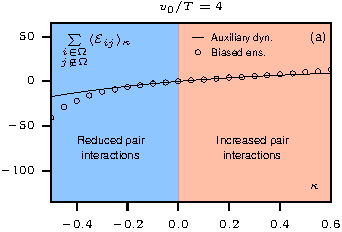
\includegraphics[width=.49\linewidth]{fig3a.pdf}
	\hfill
	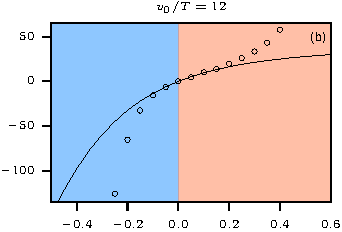
\includegraphics[width=.49\linewidth]{fig3b.pdf}
	\vskip.5cm
	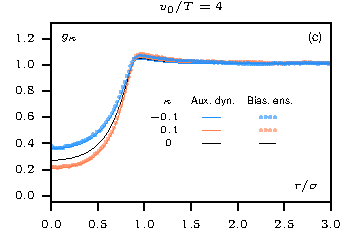
\includegraphics[width=.49\linewidth]{fig3c.pdf}
	\hfill
	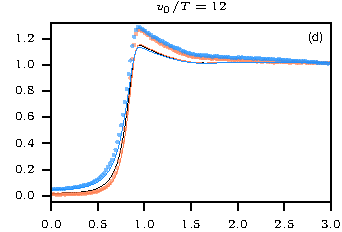
\includegraphics[width=.49\linewidth]{fig3d.pdf}
	\caption{\label{fig:energybias}
		(a-b)~Average biasing observable $\sum_{i\in\Omega,j\not\in\Omega}\langle{\cal E}_{ij}\rangle_\kappa = \sum_{i\in\Omega,j\not\in\Omega}\langle{\cal L} v({\bf r}_i-{\bf r}_j)\rangle_\kappa/T$ as a function of bias parameter $\kappa$, where ${\cal L}$ and $v$ respectively denote the evolution operator and the pair potential of the equilibrium dynamics~\eqref{eq:dyn_eq}. Results from the first-order auxiliary dynamics (solid lines) and from a direct sampling of the biased ensemble (circles) coincide for a finite range of $\kappa$.
		(c-d)~Biased density correlation $g_\kappa$ as a function of interparticle distance $r/\sigma$ obtained from auxiliary dynamics (solid lines) and direct sampling (dotted lines). At leading order, our dynamical bias effectively renormalizes the potential $v$ by a factor $\kappa$ for specific pairs of particles $\{i\in\Omega,j\not\in\Omega\}$, in satisfying agreement with direct sampling for weak interactions ($v_0=4T$). This illustrates the control of liquid structure at small $\kappa$ and weak interactions.
		Simulation details in Appendix~\ref{app:simu}.
}
\end{figure*}


The pedagogical example in Sec.~\ref{sec:biasexternal} can also be treated perturbatively using the operator formalism described above. Such calculations indeed show that the effect of applying a bias is equivalent to introducing a constant driving force at first order. Besides, the techniques in Sec.~\ref{sec:biasexternal} allow one to anticipate the trajectories generated at higher-order bias, by biasing the dynamics given by the potential~\eqref{eq:centralresult0} with 
\begin{equation}\label{eq:eps_pprime}
	\varepsilon' = \frac{1}{\gamma T}\int_0^t\sum_k\Big[\sum_{i,j}\kappa_{ij} \nabla_kv({\bf r}_i(s)-{\bf r}_j(s))\Big]^2{\rm d}s .
\end{equation}
Then, it follows that the effect of higher-order bias on trajectories amounts to maximizing the squared forces in the integrand of~\eqref{eq:eps_pprime}, which effectively tends to cluster particles for both signs of $\kappa_{ij}$.


Finally, the decomposition between first-order auxiliary potential and higher-order symmetric bias can be extended to a generic class of biases of the form $T{\cal E}_{ij} = {\cal L} A({\bf r}_i-{\bf r}_j)$ for an arbitrary observable $A$. As detailed in Appendix~\ref{app:far}, the corresponding first-order auxiliary potential $V+2\sum_{i,j}\kappa_{ij}A({\bf r}_i-{\bf r}_j)$ is now complemented with the higher-order bias~\eqref{eq:eps_pprime} where $A$ simply replaces $v$. Such a bias is reminiscent of, yet qualitatively different from, the escape rate used to promote dynamical heterogeneity in glassy systems~\cite{Pitard2011, Fullerton2013}. In our case, clustering is favored for both positive and negative bias parameters $\kappa_{ij}$. In particular, this is in contrast with the emergence of a hyperuniform phase, where large scale fluctuations are suppressed, reported when biasing some hydrodynamic theories of diffusive systems~\cite{Jack2015b}.



% -------------------------------------------------------------------------------


\begin{figure*}
	\centering
	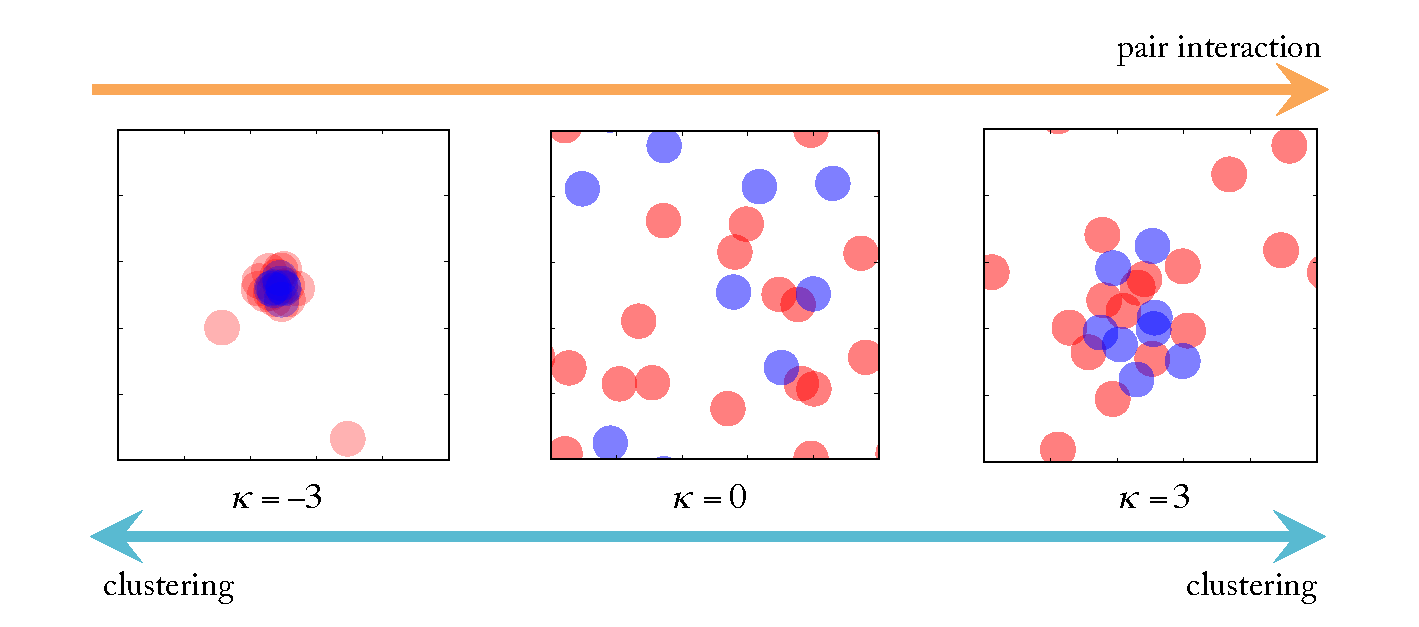
\includegraphics[width=.9\linewidth]{fig4.pdf}
	\caption{\label{fig:outofperturbation}
	Configurations obtained from a direct sampling of the biased ensemble where the interaction potential is selectively targeted for blue-red pairs of particles. The blue and orange arrows respectively indicate (i) the increased propensity to form clusters for $\kappa=\pm3$, and (ii) the increase of pair interaction strength from $\kappa=-3$ to $3$. Our bias promotes clustering with different renormalized interactions for positive and negative biases. As a result, particles aggregate either with a random composition ($\kappa=3$) or in a micelle-like structure with a blue core ($\kappa=-3$). This illustrates how biasing specific pairs leads to supervised spatial organization.
		Simulation details in Appendix~\ref{app:simu} and movies in~\cite{movie}.
	}
\end{figure*}


\subsection{{Numerical sampling of biased structures}}

To illustrate the potential of our bias to control liquid properties, we focus in what follows on the specific case $\kappa_{ij}=\kappa\delta_{i\in\Omega}\delta_{j\not\in\Omega}$ where all pairs between a subset $\Omega$ and other particles are biased with the same strength $\kappa$. Here, the set $\Omega$ could for instance refer to some tracer particles immersed in the liquid, to connect with the settings in Sec.~\ref{sec:method}. 


To confirm numerically the validity of our appraoch, we first probe the range of the first-order auxiliary dynamics where interactions {are predicted to be} simply renormalized. We compare measurements of $\sum_{i\in\Omega, j\in\Omega}\langle{\cal E}_{ij}\rangle_\kappa$, where $\langle\cdot\rangle_\kappa$ denotes an average in the biased ensemble, obtained from simulations {with} {the renormalized potentials in}~\eqref{eq:centralresult0} and from a direct sampling of the biased ensemble. The latter is implemented with a cloning algorithm which regularly selects and multiplies rare realizations for efficient sampling~\cite{Giadina2006, tailleur2007probing, Hurtado2009, Nemoto2016, Ray2018, Klymko2018, Brewer2018}. For convenience, interactions are now given by the soft-core potential $v({\bf r}) = v_0\exp\big[-1 / (1 - (|{\bf r}|/\sigma)^2)\big]\Theta(\sigma-|{\bf r}|)$. For weak interactions ($v_0=4T$), we observe a very satisfying agreement between the two measurements for a finite range of $\kappa$, as reported in Fig.~\ref{fig:energybias}(a), which supports the validity of our perturbation up to interaction change between $-20\%$ and $+40\%$. The range of validity decreases as $v_0/T$ increases, as shown in Fig.~\ref{fig:energybias}(b), and we expect a similar trend when also increasing the number of biased pairs.


To explore further the features of this biased ensemble, we now compare the density correlations of biased pairs $g_\kappa({\bf r})\sim \sum_{i\in\Omega,j\not\in\Omega}\langle \delta({\bf r}-{\bf r}_i+{\bf r}_j)\rangle_\kappa$ obtained from both direct sampling and first-order auxiliary dynamics. For $\kappa=\pm0.1$, we observe that the structural modification induced by the bias becomes more dramatic as $v_0/T$ increases. The agreement between cloning and auxiliary dynamics is good for the whole curve when $v_0/T=4$, whereas a clear deviation appears beyond $r\simeq\sigma$ when $v_0/T=12$, as shown in Figs.~\ref{fig:energybias}(c-d). In both cases, the region of particle overlap $r<\sigma$ is well reproduced. {These results corroborate the ability of the first-order auxiliary dynamics to capture interaction changes as a simple renormalization of potential strength. At variance, the tendency for particles to cluster, manifest numerically in the increased peak value at $r\simeq\sigma$, is a higher-order effect missed by this auxiliary dynamics. Yet, note that the peak value is comparable for $\kappa=\pm0.1$, in agreement with~\eqref{eq:eps_pprime} being symmetric in $\kappa$.} Altogether, these results demonstrate that our bias modulates the liquid structure in a controlled manner for small bias and weak interactions as predicted by~\eqref{eq:centralresult0}.


Finally, we probe numerically the effect of large bias ($|\kappa|>1$) using direct sampling, to explore configurations significantly distinct from the one of the equilibrium dynamics~\eqref{eq:dyn_eq}. The particles spontaneously tend to cluster for both positive and negative $\kappa$, as shown in Fig.~\ref{fig:outofperturbation} and movies in~\cite{movie}. This confirms the propensity of trajectories to maximize interaction forces at high bias, as captured by~\eqref{eq:eps_pprime}. Importantly, the shape of clusters differs depending on the sign of $\kappa$: a micelle-like structure featuring the particles in $\Omega$ at the core (blue) surrounded by others (red) appears for $\kappa=-3$, whereas clusters have a random composition for $\kappa=3$. Again, this agrees with the renormalized interactions being either increased or decreased, respectively for $\kappa>0$ and $\kappa<0$. In general, two types of configurations should generically be stabilized, for a given interaction potential $v$, depending on the sign of the bias. Overall, this establishes a reliable proof of principle for the design of tailored self-assembled structures with our specific choice of biased ensembles.

% ===============================================================================

\subsection{{Biased energy flows and flocking transitions in a Vicsek inspired model}}
As a final illustration of the effectiveness and utility of our techniques, we apply our energy flow biasing technique to a Vicsek inspired model. This model was previously studied in Ref~\cite{Farrell2012} and is composed of self propelled particles that interact according to a pairwise aligning forcing, 
\begin{equation}
    \label{eq:vicsek}
    \dot{{\bf r}}_i= v{\rm e}_{\theta_i};\dot{\theta_i}=\gamma \sum_{j=1}^{N} F(\theta_j-\theta_i,{\bf r}_i,{\bf r}_j)+\sqrt{2 \epsilon} \tilde \eta_i(t) 
\end{equation}
where ${\bf r}_i$ describes the position and $\theta_i$ describes the orientation of the $i^{\th}$ particle, $\gamma$ and $\epsilon$ describe the strength of alignment and fluctuations respectively, $N$ denotes the number of particles, $\tilde \eta(t)$ is a Gaussian white noise with unit variance and zero mean and the aligning force is given by $F(\theta,{\bf r})=\sin(\theta)/\pi R^2$ if $|{\bf r}|<R$. Following Ref~\cite{Farrell2012}, we set $R=1$. This model exhibits an disorder-order transition from an isotropic to a flocked state as $\gamma$, $\epsilon$ and the density of particles, $\rho=N/L^2$, where $L$ is the size of the simulation box, are tuned. In particular, a mean field continuum theory predicts that transition happens at a critical value of $\epsilon_c=1/2 \gamma \rho$, with the system existing in a flocked state for $\epsilon<\epsilon_c$ and the system existing in a homogeneous disordered state for $\epsilon>\epsilon_c$. 

Applying the above described energy biasing techniques to fluctuations in the orientation fields, $\theta_i$, we can effectively generate steady states with modified inter particle aligning interactions. The specific form of the biasing fucntion, $\cal E$ is derived in the appendix following a procedure analogous to the one employed above. In particular, in the limit of a small biasing field, the steady states generated under biasing will resemble the unbiased non-equilibrium steady states generated with new aligning interactions, 
\begin{equation}
\label{eq:vicsekcentral1}
\tilde F=F(1+\kappa)\,,
\end{equation}
similar to the result in ~\eqref{eq:centralresult0}. In this manner, by promoting biased energy flows, the effective aligning interactions can be tuned in a controlled manner. In Fig XXX (supplementary movies XXX), we provide qualitative results confirming our theoretical prediction. Starting with a model system with $\epsilon_c=1/2 \gamma \rho$, a flocked state or an isotropic state can be realized according to Eq.~\ref{eq:vicsekcentral1} simply by tuning $\kappa$ with all other interactions and parameters being held the same. Specifically, as predicted by our theory, a flocked state is obtained for $\kappa>0$ while an isotropic state is stabilized for $\kappa<0$. These results demonstrate that our approach can be potentially used to understand the interplay between energy flows and organization in systems beyond those considered in this manuscript. 
% ===============================================================================

\section{Conclusion}

Developing techniques to characterize and control the behavior of systems operating far from equilibrium remains a central and outstanding problem. Despite the apparently complex interplay between internal dissipation and emerging properties, we have demonstrated that tracer diffusion and density correlations can simply be connected to dissipation in driven liquids. Importantly, this opens promising perspectives to evaluate dissipation simply from the structure of the system. Inspired by recent work~\cite{Nardini2017}, one could for instance introduce a map of dissipation, directly related to the density map, to resolve spatially where energy is released in the thermostat. Though the corresponding integrated map would not cover the total dissipation, it would already provide insightful information about locations of low and high dissipation with respect to a constant background set by the squared driving amplitude.


In practice, monitoring dissipation with a well-defined parameter remains an open challenge for many-body systems. To this end, biased ensembles enable one to specify the statistics of dissipation by introducing an additional control parameter, analogously to the change from micro-canonical to canonical ensemble in equilibrium thermodynamics~\cite{Chetrite2013, Jack2010}. This is done by selecting rare noise realizations which drive the system away from typical behaviour, without introducing any driving force. Pioneering works were focused on favoring dynamical heterogeneities, without affecting the structure, of kinetically constrained models~\cite{garrahan2007, Hedges2009, Pitard2011, Speck2012, Bodineau2012a}. Yet, more recent studies have shown the potential to also modify density correlations in diffusive systems~\cite{Jack2014, Cagnetta2017, Nemoto2019}.


Using these large-deviation techniques, we have put forward a particular set of biased ensembles which allows one to regulate the liquid structure in a controlled manner. The explicit form of the bias is motivated by the relations between dissipation and structure that we have derived for driven liquids. At leading order, any bias in this class simply leads to introducing additional interactions in the dynamics. Furthermore, higher-order bias systematically constrains the trajectories to favor the formation of clusters. Based on a minimal case study, we have sampled the biased configurations, using state-of-the-art numerics~\cite{Giadina2006, tailleur2007probing, Hurtado2009, Nemoto2016, Ray2018, Klymko2018, Brewer2018}, to illustrate the ability to stabilize specific structures in a controlled manner. 


Since dynamical bias consists in favoring rare noise fluctuations, the corresponding dynamics effectively provides useful insights on how to promote atypical configurations with an external drive. In practice, the driving protocol should simply mimic the biased noise realizations. This line of thought has already been exploited for efficient sampling of the biased ensemble~\cite{Nemoto2016, Jack2017, Jack2018}, where control forces make rare events become typical. Moreover, since our analytic framework encompasses the case of a specific bias for each pair of particle, it could potentially be regarded as a fruitful route to promote the spontaneous self-assembly of complex structures at the cost of energy dissipation. For instance, inspired by recent works~\cite{Murugan2015, Murugan2017b}, one might consider our approach to design energetic landscapes, in terms of the pair-specific bias parameters, which selectively stabilize some target molecules. 


Overall, these results illustrate how specifying the amount of energy dissipated by nonequilibrium forces allows one to constrain the dynamics and structure of driven liquids. This paves the way towards controlling the emerging properties of such systems by tuning dissipation accurately. It remains to investigate whether similar results can be obtained in more complex systems, such as self-propelled particles where the driving is independent for each particle~\cite{Marchetti2013, Cates2015, Bechinger2016, Marchetti2018}, which could also potentially include anisotropic building blocks, such as driven chiral objects or active liquid crystals~\cite{Joshi2017, VanZuiden2016, Nguyen2014b}. 


% ===============================================================================


\acknowledgements{The authors acknowledge insightful discussions with Michael E. Cates, Robert L. Jack, and Vincenzo Vitelli. This work was granted access to the HPC resources of CINES/TGCC under the allocation 2018-A0042A10457 made by GENCI and of MesoPSL financed by the Region Ile de France and the project Equip@Meso (reference ANR-10-EQPX-29-01) of the program Investissements d'Avenir supervised by the Agence Nationale pour la Recherche. SV and LT were supported by the University of Chicago Materials Research Science and Engineering Center, which is funded by National Science Foundation under award number DMR-1420709. SV acknowledges support from the Sloan Foundation and startup funds from the University of Chicago. LT acknowledges support from the National Science Foundation under award number DMR-1848306. \'EF benefits from an Oppenheimer Research Fellowship from the University of Cambridge, and a Junior Research Fellowship from St Catherine's College.}


% ===============================================================================


\appendix

\section{Numerical simulations}\label{app:simu}

In Sec.~\ref{sec:map}, a custom code of molecular dynamics, based on finite time difference, is used to perform the simulations in a two-dimensional box $10^2\sigma\times 10^2\sigma$ with periodic boundary conditions. The time step is $\delta t = 10^{-4}$ and the initial condition is homogeneous. Parameter values: $\rho_0=0.7$, $T=0$, $\gamma=1$, $f=3\times 10^{-2}$, $\tau=10^3$, $v_0=5$, $n=10^2$, $\sigma=1$.


In Secs.~\ref{sec:diff} and~\ref{sec:struc}, numerical simulations of the dynamics~\eqref{eq:dyn} are performed using the LAMMPS simulation package in a two-dimensional box $10^2\sigma\times 10^2\sigma$, where $\sigma$ is the particle diameter, with periodic boundary conditions at average density $\rho_0=0.45$. The driving force ${\bf F}_{\rm d}$ only acts on ten percent of the particles with dynamics~\eqref{eq:theta}. The time step is $\delta t = 5\times 10^{-4}$. The system is first relaxed for $10^5$ time steps, and later equilibrated for $50\tau$. We evaluate average values over trajectories with duration of at least $150\tau$. Parameter values: $T=1$, $\gamma=10^2$, $v_0=1$, $\sigma=1$.


In Sec.~\ref{sec:bias}, a custom code of molecular dynamics, based on finite time difference, is used to perform the simulations in a two-dimensional box $10\sigma\times 10\sigma$ with periodic boundary conditions. The pair potential of $16$ particle pairs is biased in a system of $40$ particles in total. To sample the biased ensemble, we use the cloning algorithm described in Appendix A of~\cite{Nemoto2016}. The time interval for cloning is $\Delta t = 10 \delta t$ and the number of clones is $1600$. The time step is $\delta t = 10^{-4}$, the initial relaxation time is $10^4\Delta t$, and the total simulation time is $10^6 \Delta t$. Parameter values: $T=1$, $\gamma=1$, $v_0=4$ (Fig.~\ref{fig:outofperturbation}), $\sigma=1$.


% -------------------------------------------------------------------------------


\section{Dissipation and diffusion}\label{app:diff}

This appendix is devoted to the derivation of the dissipation rate $\cal J$ and the diffusion coefficient $D$ of a driven tracer, as defined in Sec.~\ref{sec:method}. We employ a perturbative treatment at weak interactions, originally introduced for a particle driven at constant force in~\cite{Demery2011, Demery2014}. To this aim, the tracer-bath interaction potential $v$ is scaled by a small dimensionless parameter $h\ll1$ in what follows. Besides, we focus on the regime of dilute tracers, so that interactions among them, either direct or mediated by the bath, can be safely neglected.


The dynamic action associated with the tracer dynamics~(\ref{eq:rho}-\ref{eq:EvolutionTracer}) follows from standard path integral methods~\cite{Martin1973, Dominicis1975}. It can be separated into contributions from the free tracer motion and from interactions, respectively denoted by ${\cal A}_0$ and ${\cal A}_{\rm int}$:
\begin{equation}\label{eq:action_app}
	\begin{aligned}
		{\cal A}_0 &= \int \bar{\bf r}_0 \cdot \big[ {\rm i}(\dot{\bf r}_0 - {\bf F}_{\rm d}/\gamma) + D_0 \bar{\bf r}_0 \big] {\rm d}t ,
		\\
		{\cal A}_{\rm int} &= \frac{h^2}{\gamma} \int \frac{{\rm d}{\bf q}}{(2\pi)^d} |{\bf q}|^2 |v({\bf q})|^2 \int_{-\infty}^\infty {\rm d}s\int_{-\infty}^s{\rm d}u
		\\
		&\quad\times {\rm e}^{-D_{\rm G}|{\bf q}|^2K({\bf q})(s-u)+{\rm i}{\bf q}\cdot[{\bf r}_0(s)-{\bf r}_0(u)]}
		\\
		&\quad\times \bar{\bf r}_0(s) \cdot \bigg[ \frac{\bar{\bf r}_0(u)}{\gamma K({\bf q})} - \frac{{\bf q}}{\gamma_{\rm G}} \bigg] ,
	\end{aligned}
\end{equation}
where $D_0=T/\gamma$ is the tracer diffusion coefficient in the absence of interactions ($v=0$), and $\bar{\bf r}_0$ is the process conjugated with the tracer position ${\bf r}_0$. For weak interactions $h\ll1$, any average value can be then expanded in terms of $h$ as $\langle\cdot\rangle=\langle\cdot\rangle_0 - h^2 \langle{\cal A}_{\rm int}\cdot\rangle_0 + {\cal O}(h^4)$, where $\langle\cdot\rangle_0$ is the average taken with respect to ${\cal A}_0$ only. As a result, determining the first correction from interactions in any observable amounts to computing the corresponding average $\langle{\cal A}_{\rm int}\cdot\rangle_0$.


Considering the dissipation rate ${\cal J}=\langle\dot{\bf r}_0\rangle\cdot{\bf F}_{\rm d}$, the leading order is $\langle\dot{\bf r}_0\rangle_0 \cdot {\bf F}_{\rm d} = |{\bf F}_{\rm d}|^2/\gamma = f^2/\gamma$, and the first correction reads $ - h^2 \langle{\cal A}_{\rm int}\dot{\bf r}_0\rangle_0 \cdot {\bf F}_{\rm d} $. Given the explicit form of ${\cal A}_{\rm int}$ in~\eqref{eq:action_app}, the correlations of interest are
\begin{equation}
	\begin{aligned}
		\Big\langle\dot{\bf r}_0(t) &\big[{\bf q}\cdot\bar{\bf r}_0(s)\big] {\rm e}^{{\rm i}{\bf q}\cdot[{\bf r}_0(s)-{\bf r}_0(u)]}\Big\rangle_0
		\\
		&= {\rm i}{\bf q}\delta(t-s){\rm e}^{ - D_0|{\bf q}|^2(t-u) + \frac{{\rm i}{\bf q}}{\gamma}\cdot\int_u^t {\bf F}_{\rm d}(w) {\rm d}w} ,w
		\\
		\Big\langle\dot{\bf r}_0(t) &\big[\bar{\bf r}_0(u)\cdot\bar{\bf r}_0(s)\big] {\rm e}^{{\rm i}{\bf q}\cdot[{\bf r}_0(s)-{\bf r}_0(u)]}\Big\rangle_0
		\\
		&= -{\rm i}{\bf q}\delta(t-s){\rm e}^{ - D_0|{\bf q}|^2(t-u) + \frac{{\rm i}{\bf q}}{\gamma}\cdot\int_u^t {\bf F}_{\rm d}(w) {\rm d}w} ,
	\end{aligned}
\end{equation}
where we have used that the tracer statistics is Gaussian in the absence of interactions, following~\cite{Demery2011, Demery2014}. From this result, we get
\begin{equation}
	\begin{aligned}
		&{\cal J} - f^2/\gamma
		\\
		&\,= \frac{h^2}{d\gamma^2} \int \frac{{\rm d}{\bf q}}{(2\pi)^d} {\rm i}{\bf q}\cdot{\bf F}_{\rm d}(t) |{\bf q}|^2 |v({\bf q})|^2 \frac{D_0+D_{\rm G}K({\bf q})}{D_0K({\bf q})}
		\\
		&\,\quad\times \int_{-\infty}^t {\rm d}u {\rm e}^{-|{\bf q}|^2 [D_0+D_{\rm G} K({\bf q})](t-u) + \frac{{\rm i}{\bf q}}{\gamma}\cdot\int_u^t{\bf F}_{\rm d}(w){\rm d}w}
		\\
		&\,\quad + {\cal O}(h^4) ,
	\end{aligned}
\end{equation}
where we have used $\gamma_{\rm G}=\gamma/\rho_0$ and $D_{\rm G}=\rho_0D_0$. Expanding at small $f$, we deduce
\begin{equation}\label{eq:diss}
	\begin{aligned}
		&{\cal J} - f^2/\gamma
		\\
		&\,= - \frac{h^2}{d\gamma^3} \int \frac{{\rm d}{\bf q}}{(2\pi)^d} |{\bf q}|^4 |v({\bf q})|^2 \frac{D_0+D_{\rm G}K({\bf q})}{D_0K({\bf q})}
		\\
		&\,\quad\times \int_{-\infty}^t {\rm d}u {\rm e}^{-|{\bf q}|^2 [D_0+D_{\rm G} K({\bf q})](t-u)} \int_u^t{\rm d}w{\bf F}_{\rm d}(t)\cdot{\bf F}_{\rm d}(w)
		\\
		&\,\quad + {\cal O}(h^4,f^4) .
	\end{aligned}
\end{equation}
Substituting the explicit expression of the external drive~\eqref{eq:theta} in~\eqref{eq:diss}, and then integrating over $u$ and $w$, we obtain
\begin{equation}
	\begin{aligned}
		&{\cal J} - f^2/\gamma
		\\
		&\,= - \frac{(hf)^2}{d\gamma^3} \int \frac{{\rm d}{\bf q}}{(2\pi)^d} \frac{|{\bf q}|^4 |v({\bf q})|^2}{|{\bf q}|^4\big[D_0+D_{\rm G}K({\bf q})\big]^2 + \omega^2}
		\\
		&\,\quad\times \frac{D_0+D_{\rm G}K({\bf q})}{D_0K({\bf q})} + {\cal O}(h^4,f^4) .
	\end{aligned}
\end{equation}
For the case of internal drive with correlations~\eqref{eq:theta_ac}, we exploit the equivalence with a disordered drive detailed in Sec.~\ref{sec:map}. Substituting the explicit drive~\eqref{eq:theta_dis} in~\eqref{eq:diss}, and then averaging over disorder in the limit of many oscillators ($n\gg1$), we get
\begin{equation}
	\begin{aligned}
		&{\cal J} - f^2/\gamma
		\\
		\,&= - \frac{(hf)^2}{d\gamma^3} \int \frac{{\rm d}{\bf q}{\rm d}\omega'}{(2\pi)^{d+1}} \frac{|{\bf q}|^4 |v({\bf q})|^2 \phi(\omega')}{|{\bf q}|^4\big[D_0+D_{\rm G}K({\bf q})\big]^2 + (\omega')^2}
		\\
		&\quad\times \frac{D_0+D_{\rm G}K({\bf q})}{D_0K({\bf q})} + {\cal O}(h^4,f^4) ,
	\end{aligned}
\end{equation}
where $\phi(\omega') = 2\tau/\big[1+(\omega'\tau)^2\big]$, yielding
\begin{equation}
	\begin{aligned}
		&{\cal J} - f^2/\gamma
		\\
		\,&= - \frac{\tau(hf)^2}{d\gamma^3} \int \frac{{\rm d}{\bf q}}{(2\pi)^d} \frac{|{\bf q}|^2 |v({\bf q})|^2}{D_0 K({\bf q})}
		\\
		&\quad\times \frac{1}{\tau|{\bf q}|^2\big[D_0+D_{\rm G}K({\bf q})\big] + 1} + {\cal O}(h^4,f^4) .
	\end{aligned}
\end{equation}
The asymptotic results for the rate of work $\dot w = f^2/\gamma-{\cal J}$, presented in Sec.~\ref{sec:diff} for both external and internal drivings, follow directly.


We now turn to deriving the diffusion coefficient $D$. It is defined in terms of the mean-squared displacement (MSD) $\langle\Delta{\bf r}_0^2(t)\rangle=\big\langle\big[\langle{\bf r}_0(t)\rangle - {\bf r}_0(t)\big]^2\big\rangle$ as $D=\underset{t\to\infty}{\lim}\langle\Delta{\bf r}_0^2(t)\rangle / 2 d t$. At leading order, the MSD reads $\langle\Delta{\bf r}_0^2(t)\rangle_0 = 2dD_0t$. To obtain the first order, we need to compute the following correlations
\begin{equation}
	\begin{aligned}
		\Big\langle\Delta{\bf r}^2_0(t)& \big[{\bf q}\cdot\bar{\bf r}_0(s)\big] {\rm e}^{{\rm i}{\bf q}\cdot[{\bf r}_0(s)-{\bf r}_0(u)]}\Big\rangle_0
		\\
		&= - 4 (D_0/\gamma)|{\bf q}|^2(s-u) \Theta(t-s)
		\\
		&\quad\times{\rm e}^{ - D_0|{\bf q}|^2(t-u) + \frac{{\rm i}{\bf q}}{\gamma}\cdot\int_u^t {\bf F}_{\rm d}(w) {\rm d}w},
		\\
		\Big\langle\Delta{\bf r}^2_0(t)& \big[\bar{\bf r}_0(u)\cdot\bar{\bf r}_0(s)\big] {\rm e}^{{\rm i}{\bf q}\cdot[{\bf r}_0(s)-{\bf r}_0(u)]}\Big\rangle_0
		\\
		&= (2/\gamma^2)\Theta(t-s) \big[2D_0|{\bf q}|^2(s-u)-1\big]
		\\
		&\quad\times{\rm e}^{ - D_0|{\bf q}|^2(t-u) + \frac{{\rm i}{\bf q}}{\gamma}\cdot\int_u^t {\bf F}_{\rm d}(w) {\rm d}w} ,
	\end{aligned}
\end{equation}
where we have used again that ${\cal A}_0$ is Gaussian in terms of $\bar{\bf r}_0$, yielding
\begin{equation}
	\begin{aligned}
		&\big\langle\Delta{\bf r}^2_0(t)\big\rangle - 2 d D_0 t
		\\
		&\,= \frac{2h^2}{\gamma^2} \int \frac{{\rm d}{\bf q}}{(2\pi)^d} \frac{|{\bf q}|^2 |v({\bf q})|^2}{K({\bf q})}
		\\
		&\,\quad\times \int_{-\infty}^t{\rm d}s \int_{-\infty}^s{\rm d}u \big\{ 2|{\bf q}|^2\big[D_0+D_{\rm G}K({\bf q})\big](s-u) - 1\big\}
		\\
		&\,\quad\times {\rm e}^{ -|{\bf q}|^2[D_0+D_{\rm G}K({\bf q})](s-u) + \frac{{\rm i}{\bf q}}{\gamma}\cdot\int_u^s{\bf F}_{\rm d}(w) {\rm d}w } + {\cal O}(h^4) .
	\end{aligned}
\end{equation}
Expanding at small $f$, we get
\begin{equation}
	\begin{aligned}
		&\big\langle\Delta{\bf r}^2_0(t)\big\rangle - 2 d D_{\rm eq} t
		\\
		&\,= - \frac{2h^2}{\gamma^4} \int \frac{{\rm d}{\bf q}}{(2\pi)^d} \frac{|{\bf q}|^4 |v({\bf q})|^2}{K({\bf q})}
		\\
		&\,\quad\times \int_{-\infty}^t{\rm d}s \int_{-\infty}^s{\rm d}u \big\{ 2|{\bf q}|^2\big[D_0+D_{\rm G}K({\bf q})\big](s-u) - 1\big\}
		\\
		&\,\quad\times {\rm e}^{ -|{\bf q}|^2[D_0+D_{\rm G}K({\bf q})](s-u)} \int_u^s {\rm d}w_1{\rm d}w_2 {\bf F}_{\rm d}(w_1)\cdot{\bf F}_{\rm d}(w_2)
		\\
		&\,\quad + {\cal O}(h^4,f^4) ,
	\end{aligned}
\end{equation}
where $D_{\rm eq}$ refers to the diffusion coefficient in the absence of driving force ($f=0$). For the external drive~\eqref{eq:theta}, the explicit time integrations give
\begin{equation}
	\begin{aligned}
		D - D_{\rm eq} &= \frac{(hf)^2}{d\gamma^4} \int \frac{{\rm d}{\bf q}}{(2\pi)^d} \frac{|{\bf q}|^2|v({\bf q})|^2}{K({\bf q})\big[D_0+D_{\rm G}K({\bf q})\big]}
		\\
		&\quad\times \frac{5|{\bf q}|^4\big[D_0+D_{\rm G}K({\bf q})\big]^2 + \omega^2}{ \big\{ |{\bf q}|^4\big[D_0+D_{\rm G}K({\bf q})\big]^2 + \omega^2 \big\}^2}
		\\
		&\quad + {\cal O}(h^4,f^4) .
	\end{aligned}
\end{equation}
Using the mapping in Sec.~\ref{sec:map} for the case of internal drive with correlations~\eqref{eq:theta_ac}, we deduce
\begin{equation}
	\begin{aligned}
		D - D_{\rm eq} &= \frac{(hf)^2}{d\gamma^4} \int \frac{{\rm d}{\bf q}{\rm d}\omega'}{(2\pi)^{d+1}} \frac{|{\bf q}|^2|v({\bf q})|^2\phi(\omega')}{K({\bf q})\big[D_0+D_{\rm G}K({\bf q})\big]}
		\\
		&\quad\times \frac{5|{\bf q}|^4\big[D_0+D_{\rm G}K({\bf q})\big]^2 + (\omega')^2}{ \big\{ |{\bf q}|^4\big[D_0+D_{\rm G}K({\bf q})\big]^2 + (\omega')^2 \big\}^2}
		\\
		&\quad + {\cal O}(h^4,f^4) ,
	\end{aligned}
\end{equation}
where again $\phi(\omega') = 2\tau/\big[1+(\omega'\tau)^2\big]$, yielding
\begin{equation}
	\begin{aligned}
		D - D_{\rm eq} &= \frac{\tau(hf)^2}{d\gamma^4} \int \frac{{\rm d}{\bf q}}{(2\pi)^d} \frac{|v({\bf q})|^2}{K({\bf q})\big[D_0+D_{\rm G}K({\bf q})\big]^2}
		\\
		&\quad\times \frac{5\tau|{\bf q}|^2\big[D_0+D_{\rm G}K({\bf q})\big] + 3}{ \big\{ \tau|{\bf q}|^2\big[D_0+D_{\rm G}K({\bf q})\big] + 1 \big\}^2}
		\\
		&\quad + {\cal O}(h^4,f^4) .
	\end{aligned}
\end{equation}
Finally, we obtain the expressions in the asymptotic regimes, as reported in Sec.~\ref{sec:diff} for both external and internal drivings.


% -------------------------------------------------------------------------------


\section{Equivalence of biased ensembles}\label{app:far}

In this Appendix, we demonstrate the equivalence between two dynamical biased ensembles. Ensemble~(a) corresponds to the equilibrium dynamics~\eqref{eq:dyn_eq} biased with the factor $\exp\big[\sum_{i,j} \kappa_{ij}\int_0^t{\cal E}_{ij}(s){\rm d}s\big]$ in the path probability, where
\begin{equation}
	{\cal E}_{ij} = \frac{1}{\gamma T} \sum_k\big[T\nabla_k - \nabla_kV\big]\cdot\nabla_k A({\bf r}_i-{\bf r}_j) .
\end{equation}
Ensemble~(b) is associated with the first-order auxiliary dynamics, whose potential reads $V+2\sum_{i,j}\kappa_{ij}A({\bf r}_i-{\bf r}_j)$, biased with
\begin{equation}
	\varepsilon' = \frac{1}{\gamma T}\int_0^t\sum_k\Big[\sum_{i,j}\kappa_{ij} \nabla_kA({\bf r}_i(s)-{\bf r}_j(s))\Big]^2{\rm d}s .
\end{equation}
Obtaining the equivalence between (a) and (b) amounts to showing that their path probabilities are similar. The corresponding dynamic actions, denoted by ${\cal A}^{( \sigma)}(t) = \sum_k\int_0^t{\mathbb A}_k^{(\sigma)}(s){\rm d}s$ for $\sigma=\{{\rm a,b}\}$, are given by
\begin{equation}
	\begin{aligned}
		{\mathbb A}_k^{(\rm a)} &= \frac{1}{4\gamma T} \big[\gamma\dot{\bf r}_k + \nabla_kV\big]^2 - \frac{1}{2\gamma} \nabla^2_kV
		\\
		&\quad - \frac{1}{\gamma T} \sum_{i,j}\kappa_{ij}\big[T \nabla_k - \nabla_k V\big] \cdot\nabla_k A({\bf r}_i-{\bf r}_j) ,
		\\
		{\mathbb A}_k^{(\rm b)}	&= \frac{1}{4\gamma T} \Big[\gamma\dot{\bf r}_k + \nabla_k V + 2\sum_{i,j}\kappa_{ij}\nabla_kA({\bf r}_i-{\bf r}_j)\Big]^2
		\\
		&\quad - \frac{1}{2\gamma} \nabla^2_k \Big[V + 2\sum_{i,j}\kappa_{ij} A({\bf r}_i-{\bf r}_j)\Big]
		\\
		&\quad - \frac{1}{\gamma T}\Big[\sum_{i,j}\kappa_{ij}\nabla_kA({\bf r}_i-{\bf r}_j)\Big]^2 .
	\end{aligned}
\end{equation}
Expanding ${\mathbb A}_k^{(\rm b)}$, it appears that ${\cal A}^{(\rm a)}$ and  ${\cal A}^{(\rm b)}$ are indeed equal up to a boundary term proportional to $\sum_{i,j}\kappa_{ij}\big[A({\bf r}_i(t)-{\bf r}_j(t)) - A({\bf r}_i(0)-{\bf r}_j(0))\big]$ which can be neglected at large $t$.


% ===============================================================================


%\bibliographystyle{apsrev4-1}
\bibliography{Driven_references.bib}

\end{document}


